%% 
%% Copyright 2007, 2008, 2009 Elsevier Ltd
%% 
%% This file is part of the 'Elsarticle Bundle'.
%% ---------------------------------------------
%% 
%% It may be distributed under the conditions of the LaTeX Project Public
%% License, either version 1.2 of this license or (at your option) any
%% later version.  The latest version of this license is in
%%    http://www.latex-project.org/lppl.txt
%% and version 1.2 or later is part of all distributions of LaTeX
%% version 1999/12/01 or later.
%% 
%% The list of all files belonging to the 'Elsarticle Bundle' is
%% given in the file `manifest.txt'.
%% 
%% Template article for Elsevier's document class `elsarticle'
%% with harvard style bibliographic references
%% SP 2008/03/01

\documentclass[preprint,12pt,authoryear,titlepage]{elsarticle}

%% Use the option review to obtain double line spacing
%% \documentclass[authoryear,preprint,review,12pt]{elsarticle}

%% Use the options 1p,twocolumn; 3p; 3p,twocolumn; 5p; or 5p,twocolumn
%% for a journal layout:
%% \documentclass[final,1p,times,authoryear]{elsarticle}
%% \documentclass[final,1p,times,twocolumn,authoryear]{elsarticle}
%% \documentclass[final,3p,times,authoryear]{elsarticle}
%% \documentclass[final,3p,times,twocolumn,authoryear]{elsarticle}
%% \documentclass[final,5p,times,authoryear]{elsarticle}
%% \documentclass[final,5p,times,twocolumn,authoryear]{elsarticle}

%% For including figures, graphicx.sty has been loaded in
%% elsarticle.cls. If you prefer to use the old commands
%% please give \usepackage{epsfig}

%% The amssymb package provides various useful mathematical symbols
\usepackage{amssymb,linguex,url,color,amsmath,booktabs}
%% The amsthm package provides extended theorem environments
%% \usepackage{amsthm}

%% The lineno packages adds line numbers. Start line numbering with
%% \begin{linenumbers}, end it with \end{linenumbers}. Or switch it on
%% for the whole article with \linenumbers.
%\usepackage{lineno}
%\modulolinenumbers[5]

\usepackage{etoolbox}% http://ctan.org/pkg/etoolbox
% Update first horizontal rule to insert a \clearpage
\makeatletter
\patchcmd{\pprintMaketitle}% <cmd>
  {\hrule\vskip12pt}% <search>
  {\clearpage\hrule\vskip12\p@}% <replace>
  {}{}% <success><failure>
% Update second horizontal rule to insert a \clearpage
\patchcmd{\pprintMaketitle}% <cmd>
  {\hrule\vskip12pt}% <search>
  {\hrule\clearpage}% <replace>
  {}{}% <success><failure>
\makeatother

\linespread{1.25}

\definecolor{Green}{RGB}{10,200,100}
\newcommand{\ndg}[1]{\textcolor{Green}{[ndg: #1]}}  
\newcommand{\gcs}[1]{\textcolor{blue}{[gcs: #1]}} 

\newcommand{\sem}[1]{\mbox{$[\![$#1$]\!]$}}

\newcommand{\lam}{$\lambda$}

\journal{Cognition}

\begin{document}

\begin{frontmatter}

%% Title, authors and addresses

%% use the tnoteref command within \title for footnotes;
%% use the tnotetext command for theassociated footnote;
%% use the fnref command within \author or \address for footnotes;
%% use the fntext command for theassociated footnote;
%% use the corref command within \author for corresponding author footnotes;
%% use the cortext command for theassociated footnote;
%% use the ead command for the email address,
%% and the form \ead[url] for the home page:
%% \title{Title\tnoteref{label1}}
%% \tnotetext[label1]{}
%% \author{Name\corref{cor1}\fnref{label2}}
%% \ead{email address}
%% \ead[url]{home page}
%% \fntext[label2]{}
%% \cortext[cor1]{}
%% \address{Address\fnref{label3}}
%% \fntext[label3]{}

%%\title{Resolving uncertainty in plural predication}

%% use optional labels to link authors explicitly to addresses:
%% \author[label1,label2]{}
%% \address[label1]{}
%% \address[label2]{}

\title{Resolving uncertainty in plural predication\tnoteref{label1}}
\tnotetext[label1]{This work was supported in part by a James S.~McDonnell Foundation Scholar Award (to N.D.G.); Office of Naval Research Grant N000141310788 (to N.D.G.); and the DARPA Probabilistic Programming for Advanced Machine Learning (PPAML) program, agreement number FA8750-14-2-0009 (to N.D.G.).}


%\author{Gregory Scontras\corref{cor1}, Noah D.~Goodman}
%\cortext[cor1]{Corresponding author}
%\ead{scontras@stanford.edu}
%\ead[url]{http://web.stanford.edu/~scontras/}
%%\author[stanford]{Noah D.~Goodman}
%\address{Stanford University}
%
%\address{Department of Psychology, Stanford University, 450 Serra Mall, Jordan Hall, Stanford, CA 94305}

%\author{Noah D.~Goodman}
%\fntext[label2]{test}

%\author{Author One\corref{cor1}\fnref{fn1}}
%\ead{email@uni.edu}
%\cortext[cor1]{Corresponding author}
%\fntext[fn1]{Student}
%
%
%\author{Author Two\fnref{fn2}}
%\ead{email2@uni.edu}
%\fntext[fn2]{Lecturer}
%
%\address{Address Here}

\author{Gregory Scontras\corref{cor1}}
\ead{scontras@stanford.edu}
\ead[url]{http://web.stanford.edu/~scontras/}
\author{Noah D.~Goodman\corref{cor2}}
\cortext[cor1]{Corresponding author}
    
 \address{Stanford University}

%% \fntext[label3]{}

\begin{abstract}
%% Text of abstract
This paper investigates the role of context in the disambiguation between distributive and collective interpretations of plural predications.  We focus on the phenomenon of ``stubborn distributivity,'' whereby certain predicates (e.g., \emph{big}, \emph{tall}) are claimed to lack collective interpretations altogether. Over the course of three experiments, we show that stubbornly distributive predicates are so because the collective properties they name are unpredictable, or unstable, in most contexts; this unpredictability results in a noisy collective interpretation, something speakers and listeners recognize as ineffective for communicating efficiently about their world.
We formalize the pragmatics of utterance disambiguation within the Bayesian Rational Speech-Acts framework, showing how stubborn distributivity emerges from properties of context and the reasoning processes of speakers and listeners: speakers prefer more stable, more potentially informative utterances; listeners understand speakers’ preferences and use this understanding as they interpret utterances.\\

\end{abstract}

\begin{keyword}
%% keywords here, in the form: keyword \sep keyword
plurality \sep distributive vs.~collective interpretations \sep ambiguity resolution \sep Rational Speech-Act models

%% PACS codes here, in the form: \PACS code \sep code

%% MSC codes here, in the form: \MSC code \sep code
%% or \MSC[2008] code \sep code (2000 is the default)

\end{keyword}

\end{frontmatter}

%\clearpage

%\linenumbers

%% main text
\section{Introduction}

If we hear ``the boys carried a piano,'' they likely carried one piano together; if we hear ``the pianos are big'' then likely each one is big. How do we understand the meaning of \emph{plural predications} like these?

The semantics and pragmatics of predicating properties to singular individuals (e.g., ``The box is big'') is already a complicated endeavor. What does it mean for a box to be big, or tall, or heavy? How do we represent its size or height or weight? Recent answers to these sorts of questions highlight the central role of context in the calculus of meaning: what properties get ascribed depend crucially on the context of predication \citep[cf.~tall for a boy vs.~tall for a basketball player;  e.g.,][]{kennedy1999,lassitergoodman2013}. The complexity associated with answering these questions increases once we introduce pluralities into the mix. 
%: however difficult the singular case, the plural case is at least $n$ times as complicated, for the $n$ many individuals under consideration. 
Particularly puzzling is the distributive vs.~collective ambiguity of plural predcation \citep[e.g.,][]{link1983,link1987,link1998,scha1984,landman1989,landman1989b,landman1996,lasersohn1988,lasersohn1990,lasersohn1995,lasersohn1998,schwarzschild1994,schwarzschild1996}:

\ex. \label{boxes} The boxes are heavy.
\a. \label{boxeseach} The boxes each are heavy. \hfill \textsc{distributive}
\b. \label{boxestogether}The boxes together are heavy. \hfill \textsc{collective}

When hearing \Last, we may infer that each box on its own counts as heavy, as in \Last[a], or only that their total weight is heavy, as in \Last[b]. Under a collective interpretation, many light boxes may together count as heavy \citep{scha1984}.
How is the interpretation determined?

Consider the well-documented yet poorly understood phenomenon of ``stubborn distributivity'' \citep{quine1960,schwarzschild2011,vazquezrojas2012,zhang2013,syrett2015}, whereby some predicates (e.g., \emph{heavy}, \emph{expensive}, \emph{voluminous}) readily admit collective construals, whiles others (e.g., \emph{big}, \emph{tall}, \emph{round}) do not. 
%When complaisantly collective gradable predicates like \emph{heavy} (also \emph{expensive}, \emph{voluminous}) are used in plural predications the meaning is ambigious. Under a distributive reading, \ref{boxeseach}, the relevant property gets ascribed to each member of the plural subject. Under a collective reading, \ref{boxestogether}, we ascribe the property to the subject as a whole---in the case of \ref{boxes} commenting on the total weight of the boxes; many light boxes may together count as heavy \citep{scha1984}.
%The collective interpretation available to \emph{heavy} proves elusive for most other gradable predicates. 
For instance, a speaker is hard-pressed to use the sentence in \Next to say of the boxes that their total size is large.

\ex. The boxes are big.
\a. The boxes each are big. \hfill \textsc{distributive}
%\z. \emph{but not}
\b. The boxes together are big. \hfill \ding{55}\textsc{collective}

Size and shape adjectives 
%(e.g., \emph{tall}, \emph{long}, \emph{round}) 
resist collective interpretations. \cite{schwarzschild2011} terms them ``stubbornly distributive,'' signaling the lack of collective interpretations. \citet{zhang2013} labels this class of predicates ``delimitable,'' highlighting their usage to describe physical extents. Supporting the robustness of this phenomenon, \cite{syrett2015} finds evidence of stubborn distributivity in children as young as 3 years of age.

Collective predication arises when a property is ascribed directly to a plurality, rather than distributed among its members \citep{link1983}. Semanticists treat stubborn distributivity as a lexical distinction: stubbornly distributive predicates behave as such because they cannot contain pluralities in their basic denotations \citep{schwarzschild2011,vazquezrojas2012,zhang2013}.\footnote{In his characterization of stubborn distributivity, Schwarzschild first assumes that gradable adjectives are predicates of events \citep[e.g.,][]{higginbothamschein1989}. Thus, \emph{heavy} predicates over \textsc{heavy} events, \emph{big} over \textsc{big} events, etc. For \citeauthor{schwarzschild2011}, stubbornly distributive predicates are those that require their events to have only single participants. The details are not directly relevant for our purposes; what is relevant is the lexical distinction \citeauthor{schwarzschild2011} and others make between stubbornly distributive and complaisantly collective predicates.}
This explanation suffers two flaws:
First, it hypothesizes a categorical distinction that may not hold; in Expt.~2, we find a gradient of collectivity, with no clear boundary.
Second, it leaves unexplained why some predicates would contain pluralities and others not---is there a deeper explanation in terms of the properties named?

We suggest that the key underlying notion is the stability or \emph{contextual predictability} of a property when applied to a collection.
That is, there are aspects of context that affect the computation of collective properties, over and above those that affect the individual properties; when there is more uncertainty about these aspects of context, the collective property is less stable.
For instance, collective \emph{tall} names the vertical extent of a set of objects, and can vary dramatically with their arrangement.
In contrast, collective \emph{heavy} names the total weight of a set of objects, which does not vary with arrangement. 
If the precise arrangement is not in common ground, then the collective use of \emph{tall} would be more likely to mislead a listener than that of \emph{heavy}---in contrast, the distributive meaning of each predicate is fully specified, independent of arrangement. A listener would thus not expect a cooperative speaker to intend the collective meaning of \emph{tall}.

Here is the general hypothesis: computing the meaning of a collective interpretation is susceptible to a varying amount of noise depending on the contextual predictability of the property at issue.
To communicate effectively and avoid possible confusion, collective interpretations will be avoided by speakers in the case of such noisy predicates; distributive interpretations, being less variable, are the safe bet. 
Listeners know this, hence collective interpretations will become more likely as contextual predictability of the collective property increases.
In section \ref{model}, we formalize the notion of contextual predictability of the collective property, and its role in the pragmatic disambiguation of the meaning of a plural predication.
This account explains the phenomenon of stubborn distributivity as a result of the relative unpredictability of the collective property for predicates like \emph{big} and \emph{tall}.
It also predicts that context should matter: in a context where the collective property is more stable, the collective reading should be more felicitous.

For physical properties, the stability of physical arrangements is a key element of context. If arrangements are less likely to change, collective properties become more predictable, and so collective interpretations become more useful and more likely. 
We test this prediction in Expt.~3, measuring whether collective \emph{big} and \emph{tall} indeed feel more natural for boxes that are always stacked regularly than for jumbled piles of boxes.
More generally, some types of objects may have more predictable collective properties than others by virtue of how regularly they instantiate in the world.  If we could find objects that instantiate in regular physical arrangements (e.g., shelves or waves) or with no physical arrangement at all (e.g., numbers or ideas), we might expect stubbornly distributive predicates to more readily admit collective interpretations when the nouns that name these objects serve as subject.
This reasoning leads to the prediction that the nouns which serve as objects in a plural predication should also affect the likelihood of collective interpretation. %\ndg{put an example back here?}
In Expt.~2, we test whether this holds for a variety of predicates.

%We are arguing for an explanation of plural predication in which ambiguity is resolved by pragmatic reasoning: the usefulness of each reading is determined partly by its contextual predictability, and readings which would be more useful on these grounds are preferred. 
Beyond contextual predictability of collective properties, the pragmatic view of plural predication entails that other standard pragmatic pressures should come to bear on the reasoning processes of speakers and listeners, affecting the felicity and thereby likelihood of the collective (and distributive) interpretation.
To whit, changing the speaker's epistemic state ought to influence the resulting disambiguation between distributive and collective interpretations. 
If a speaker lacks evidence that would verify a specific interpretation, and if a listener knows this about the speaker, then that unsupported interpretation should be particularly improbable. This intuition derives straightforwardly from the Maxim of Quality from \cite{grice1975}: ``Do not say that for which you lack adequate evidence.'' 
We test this prediction first in Expt.~1 and then with a more sensitive measure in Expt.~3.

%\gcs{this paragraph feels out of place, but I don't know where else to put it..}
%To understand more precisely why and how context  influences the interpretation of plural predication, we formalize its contribution under a pragmatic account of ambiguity resolution in section \ref{model}, using a variant of the Rational Speech-Acts model \citep[e.g.,][]{frankgoodman2012,lassitergoodman2013}. The model explains the patterns of our data well, supporting the underlying hypothesis.

Before testing the predictions of our pragmatic account, we must establish a way of studying plural predication experimentally; that is, a way to unambiguously access distributive vs.~collective interpretations. To that end, in Expt.~1, we show that the particles \emph{each} and \emph{together} reliably disambiguate plural predication. 










%%%%%%%%%%%%%%%%%%%%

%Current descriptions of the phenomenon treat it as a simple lexical distinction, an accident of semantics. 
%\ndg{here briefly note the observation that happily collective properties tend to have stable collective measures...}
%We will see, however, that the role of context in plural predication provides a ready explanation of stubborn distributivity in terms of the predictability, or subjectivity, of the collective reading. 
%More generally, we take as our motivation the idea that context plays \emph{the} key role in disambiguation for distributive vs.~collective interpretations. We consider context at three levels: 1) the immediate linguistic context (e.g., the predicate and its plural subject), 2) the specific discourse context (e.g., the epistemic states of speakers and listeners), and 3) the broader world context (e.g., information about the properties under discussion and the objects said to hold them). \ndg{smooth out this paragraph some more..}
%
%To address the issue of how (and how much) plural predication depends on context, we establish a way of studying plural predication experimentally. In Expt.~1, we introduce and validate a new methodology, which probes possible interpretations with unambiguous paraphrases. The results of Expt.~1 demonstrate a difference between \emph{big} and \emph{heavy}, as expected, but unexpectedly the stubbornly distributive predicate \emph{tall} patterns with \emph{heavy} in its ability to yield collective interpretations. We take these findings as evidence that stubborn distributivity might not be so stubborn after all, and that simple lexical distinction fails to do justice to the facts. %If it could, we should find \emph{tall} patterning with \emph{big}.
%
%We extend our paraphrase methodology in Expt.~2 to naturally-occurring examples of plural predication from the British National Corpus and the Google Books Corpus. As in Expt.~1, we continue to observe the complaisant collectivity of \emph{heavy}. However, the role of context comes more sharply into focus: with subject nouns naming objects that suggest a contextually stable collective property (i.e., a predictable collective size or shape), stubbornly distributive \emph{small} and \emph{big} yield greater rates of collective interpretations. 
%
%Following up on our corpus findings, we then explore the idea that contextual predictability of the relevant collective property is a critical factor in determining which reading is intended. Expt.~3 uses the paraphrase endorsement methodology to show that less variable contexts increase the predictability of potentially noisy collective interpretations%(e.g., always stacking objects on top of each other, regularizing the collective height of sets)
%, and, as a result, make collective interpretations more probable. 


%Still, we do our best. What follows is a brief summary of some of the progress made in understanding the semantics and pragmatics of plurality, specifically as it relates to ambiguity and the semantics of gradability. As we shall see, 


%Some predicates are inherently distributive; these are singular-seeking predicates like \emph{die} or \emph{see} or \emph{have blue eyes}; also, \emph{man}. These predicates entail a distributive reading whenever they are used: the sentence \emph{Mary and Sue saw the giraffe} entails that each of Mary and Sue saw the giraffe; \emph{John and Bill are men} entails that each of John and Bill is a man.
%Formally, inherently distributive predicates apply only to singular individuals, and refuse pluralities from their basic denotations \citep{link1983}.
%
%But not all predicates need be distributive. To illustrate this fact, \cite{link1983} reproduces the following exchange between the German newspaper \emph{Frankfurter Allgemeine Zeitung} (FAZ) and the editor of \emph{Der Speigel}, Rudolf Augstein (RA): 
%
%\ex. FAZ: ``Which property do you appreciate most with your friends?''\\
%RA: ``That they are few.''
%
%Being few is not a property any one of RA's friends holds. In fact, it makes no sense to say of an individual that he or she is few. Rather, the friends {collectively} hold this property. \citeauthor{link1983} models this fact by assuming that the predicate \emph{be few} contains in its basic denotation \emph{only} pluralities of individuals.  According to the liturgy, distributive, singular-seeking predicates and collective, plurality-seeking predicates self-sort on conceptual grounds: being a man is a property that necessarily applies to singular individuals, while being few or gathering together are properties that cannot apply to singular individuals. 
%
%Some predicates are truly ambiguous, neither inherently distributive nor inherently collective. In uttering \emph{built a raft}, we are not \emph{a priori} committed to a specific interpretation: \Next could mean either distributive \Next[a] or collective \Next[b]. Without overt linguistic or contextual cues, the meaning of the bare predicate in is underdetermined.
%
%\ex. Bill and Charlie built a raft.
%\a. Bill and Charlie each built a raft. \hfill \textsc{distributive}
%\b. Bill and Charlie together built a raft. \hfill \textsc{collective}
%
%To better understand the factors that go into the disambiguation of mixed predicates like \emph{build a raft}, we consider in detail a specific class of predicates with more concrete, (relatively) objective evaluation strategies: gradable adjectives like \emph{heavy} or \emph{big}.%\footnote{This is not to say that we know nothing about collective action statements. For example, Margaret Gilbert's Plural Subject Theory makes great gains on this ground in the domain of social philosophy \citep[for a recent overview, see][]{gilbert2013}.} 
%The measurement inherent to the semantics of these predicates delivers scalar interpretations that are amenable to quantitative study. By examining intuitions about the use of these predicates, together with the predication context that delivers them, we stand to better understand the mechanism of plural predication: when collective interpretations are appropriate, what they communicate, and what mediates the choice between distributive and collective interpretations in the first place.
%
%\subsection{Stubborn distributivity}
%
%\section{The puzzle: Stubborn distributivity}
%
%When complaisantly collective gradable predicates like \emph{heavy} (also \emph{expensive}, \emph{voluminous}) are used in plural predications the meaning is ambigious. Under a distributive reading, \ref{boxeseach}, the relevant property gets ascribed to each member of the plural subject. Under a collective reading, \ref{boxestogether}, we ascribe the property to the subject as a whole---in the case of \ref{boxes} commenting on the total weight of the boxes; many light boxes may together count as heavy \citep{scha1984}.
%
%%\ex. The boxes are heavy.
%%\a. The boxes each are heavy. \hfill \textsc{distributive}
%%\b. The boxes together are heavy. \hfill \textsc{collective}
%
%%In this latter case, where we collectively ascribe a gradable property directly to a plurality, the resulting interpretation involves sum-based aggregation strategies: if a set of boxes together holds the property of being heavy, it follows that their total weight counts as heavy \citep{scha1984}.\footnote{For now we set aside the possibility of mean-based aggregation strategies, demonstrated for plural comparisons of size by \cite{scontrasetal2012}. Given the effect of contextual predictability on sum-based aggregation strategies that we herewith elucidate, the previously demonstrated mean-based strategies likely result from an experimental context that suggested collective interpretations for \emph{bigger} and a recognition on the part of participants that average size was sufficiently predictable in that context. \ndg{perhaps move this to discussion and discuss more transparently?}} The reading becomes more transparent when we add a collective particle like \emph{together}, as in \Last[b]. Crucially, a collective reading can be true when the distributive reading is false: many light boxes may together count as heavy. These two diverging interpretations suggest a semantics for the gradable predicate \emph{heavy} under which it applies both to singular objects and pluralities in its basic denotation; it is a mixed predicate (cf.~the example \emph{build a raft} from \citealp{link1983}). 
%
%The collective interpretation available to \emph{heavy} proves elusive for most other gradable predicates. A speaker is hard-pressed to use the sentence in \Next to say of the boxes that their total size is large.
%
%\ex. The boxes are big.
%\a. The boxes each are big. \hfill \textsc{distributive}
%%\z. \emph{but not}
%\b. The boxes together are big. \hfill \ding{55}\textsc{collective}
%
%Size and shape adjectives (e.g., \emph{tall}, \emph{long}, \emph{round}) resist collective interpretations. \cite{schwarzschild2011} terms them ``stubbornly distributive,'' signaling the lack of collective interpretations. \citet{zhang2013} labels this class of predicates ``delimitable,'' highlighting their usage to describe physical extents. Supporting the robustness of this phenomenon, \cite{syrett2015} finds evidence of stubborn distributivity in children as young as 3 years of age.
%
%%In his discussion of the contrast, \citet{quine1960} describes stubbornly distributive predicates like \emph{big} in \Last as ``not cumulative,'' drawing a parallel with the nominal domain: just as a count noun like \emph{boxes} insistently ``divides its reference'' among individual boxes (in contrast to mass nouns like \emph{water} which are aggressively cumulative, referring to maximal salient quantities of water), so too do stubbornly distributive predicates divide their predication to individuals. \citeauthor{quine1960}'s characterization of the phenomenon prefigures the formal semantics that follows him. 
%
%Collective predication arises when a property is ascribed directly to a plurality, rather than distributed among its members \citep{link1983}. Semanticists hold that stubbornly distributive predicates behave as such because they cannot contain pluralities in their basic denotations \citep{schwarzschild2011,vazquezrojas2012,zhang2013}.\footnote{In his characterization of stubborn distributivity, Schwarzschild first assumes that gradable adjectives are predicates of events \citep[e.g.,][]{higginbothamschein1989}. Thus, \emph{heavy} predicates over \textsc{heavy} events, \emph{big} over \textsc{big} events, etc. For \citeauthor{schwarzschild2011}, stubbornly distributive predicates are those that require their events to have only single participants. The details are not directly relevant for our purposes; what is relevant is the lexical distinction \citeauthor{schwarzschild2011} and others make between stubbornly distributive and complaisantly collective predicates.}
%This explanation suffers two flaws:
%First, it hypothesizes a categorical distinction that may not hold; in Expt.~2 we find a gradient of collectivity, with no clear boundary.
%Second, it leaves unexplained why some predicates would contain pluralities and others not---is there a deeper explanation in terms of the properties named?
%%stating that stubbornly distributive predicates do not compose with pluralities serves merely to describe the phenomenon, not to explain it.
%%Something about these predicates, or the properties they name, must determine their behavior in plural predication. The task at hand is to determine what that thing is. 
%
%
%%Since \cite{link1983}, semanticists have been aware of necessarily distributive predicates like \emph{have blue eyes} or \emph{be a man}.  \ndg{awk} Having blue eyes or being a man are properties that necessarily hold of individuals, hence their mandatory distributivity. But collective size is not such a property, at least not transparently so. There is no conceptual barrier to attributing some size directly to a plurality of individuals. Collective nouns bring this point into focus: if a group of men has blue eyes, then each member must; if a pile of boxes counts as tall, we make no direct claim about individual box heights.
%%\ex. \a. The group of men has blue eyes. 
%%\b. The pile of boxes is tall.
%
%%\subsection{The role of context in plural predication}
%
%
%%We have seen that predicates like \textit{heavy} admit both distributive and collective interpretations: \textit{the boxes are heavy} can mean either that each member of some salient set of boxes is heavy (distributive), or that, taken together, the whole set counts as heavy (collective; \citealp{scha1984}). Crucially, the set of boxes may count as collectively heavy even when each individual box counts as light. In such a scenario, distributive and collective interpretations pull apart, suggesting a genuine ambiguity in plural predication.
%
%%Not all predicates are so permissive in their interpretations: \textit{the boxes are big} is said to communicate only about individual box size; the collective interpretation whereby speakers communicate about total set size is claimed to be absent (or at least extremely hard to come by). Other size and shape predicates are said to behave similarly.
%
%%Understanding why (and whether) stubbornly distributive predicates like \emph{big} pattern separately from what we will call ``complaisantly collective'' predicates like \emph{heavy} requires a closer look at the differences between these classes of predicates. 
%We suggest that the key underlying notion is the stability or \emph{contextual predictability} of a property when applied to a collection.
%\ndg{need to define contextual predictability clearly here. say it's a property of the denotation, not the ambiguous surface form.}
%For instance, collective \emph{tall} names the vertical extent of a set of objects, and can vary dramatically with their arrangement.
%In contrast, collective \emph{heavy} names the total weight of a set of objects, which doesn't vary with arrangement. 
%If the precise arrangement is not in common ground then the collective use of \emph{tall} would be more likely to mislead a listener than that of \emph{heavy} (in contrast, the distributive meaning of each is specified, independent of arrangement). A listener would thus not expect a cooperative speaker to intend the collective meaning of \emph{tall}.
%%Many aspects of a predicate's meaning, beyond arrangement, could give rise to similar effects
%
%%One difference between complaisantly collective \emph{heavy} and stubbornly distributive \emph{big} is the contextual predictability of the collective properties they name: the former names a maximally stable and predictable property, collective weight; to change the collective weight of a set, one would have to change the weight of an individual member. In contrast, \emph{big} names a collective property that could change with every new arrangement of the individuals said to hold it. 
%
%%The instability inherent to the collective properties named by stubbornly distributive predicates, instability that we are attuned to given our knowledge of the broader world context (i.e., knowledge of how the properties behave), supplies a ready split between these two classes of predicates. Where a property is less predictable on the basis of context, collective interpretations are noisier---they require more coordination between speakers and listeners to arrive at the same judgments about the property of interest. When coordination fails, miscommunication arises.
%
%%Consider the complaisantly collective predicate \emph{heavy}, which names the property of being heavy. 
%%With a plural subject under a collective construal, \emph{heavy} comments on total set weight.  Suppose we encounter a set of boxes piled one on top of the other. Those boxes will have a collective weight, and depending on that weight those boxes may or may not count as collectively heavy. Now, suppose we encounter that same set of boxes, this time lined up one next to the other. Despite changing the physical arrangement of the set of boxes, their weight remains the same.  Collective weight is a stable property of sets. Another complaisantly collective predicate, \emph{voluminous}, behaves similarly: the volume of a set of objects remains unchanged despite varying physical arrangement. So too for \emph{expensive} and any other complaisantly collective gradable predicate: the collective property is regular and predictable on the basis of context; rearranging the members of a plurality has no effect on the collective property itself.
%
%%Next, consider the stubbornly distributive predicate \emph{big}. Unlike with \emph{heavy}, the collective property named by \emph{big} (i.e., collective size) will depend crucially on the physical arrangement of the boxes said to hold it. Suppose we evaluate collective size by determining area in a 2D plane.\footnote{Indeed, there are many ways to evaluate the property of collective size: we could measure the total space some objects take up (including negative space), the volume the objects displace, their total width, their height, etc. This indeterminacy of dimension also contributes to the decreased contextual predictability of collective size.} Collective size does not persist against a changing arrangement of the set of boxes; change the physical arrangement of the set, and you will have changed its collective size. In many cases, for speakers and listeners to arrive at the same judgments about collective size, they need to encounter the same arrangement of objects. The same applies to the other properties named by stubborn distributive predicates, properties of physical extent.
%
%%Here it bears noting that the divide between stubbornly distributive and complaisantly collective predicates might not be so sharp as the comparison between \emph{heavy} and \emph{big} suggests. Take \emph{tall}. The predicate suggests a single, canonical strategy for evaluation: distance from the ground. However, the property does not persist despite changing physical arrangement: changing the arrangement of a set potentially changes its total distance from the ground. Still, encountering a set of boxes, it often feels perfectly felicitous to discuss their collective height using a sentence like \emph{The boxes are tall}. But note that crucial to the collective interpretation of this sentence is a specific and salient physical arrangement of boxes; an abstract set of boxes does not hold the property of being tall, but some specific arrangements of it might.
%
%%We appear to have a continuum of stubborn distributivity, or, perhaps better put, a continuum of collectivity for gradable predicates. At issue is the contextual predictability of the collective property these predicates name, which determines how noisy the collective interpretations will be. Where a property is less predictable on the basis of context, collective interpretations are noisier---they require more coordination between speakers and listeners to arrive at the same judgments about the property of interest. When coordination fails, miscommunication arises. %In other words, our---speakers' and listeners'---judgments about the truth of a collective interpretation might not align for stubbornly distributive predicates if we do not encounter the same arrangement of individuals. 
%%Noisy collective interpretations are less useful at communicating the speaker's intended message; they should therefore be less likely. With complaisantly collective predicates, the named properties are maximally predictable and therefore their collective interpretations are minimally noisy. These interpretations are therefore more likely.
%
%Here is the general hypothesis: collective interpretations are susceptible to varying amounts of noise depending on the contextual predictability of the property at issue.
%%; less predictable collective properties yield noisier collective interpretations because judgments by speakers and listeners might not align. 
%%Language is used to communicate. Speakers aspire toward clarity in this process of communication. 
%%With a stubbornly distributive predicate, the property a speaker makes reference to might change depending on the arrangement of the things said to hold it. 
%To communicate effectively and avoid possible confusion, collective interpretations will be avoided by speakers in the case of such noisy predicates; distributive interpretations being less variable are the safe bet. 
%Listeners know this, hence collective interpretations will become more likely as contextual predictability of the collective property increases.
%This would explain the phenomenon of stubborn distributivity in terms of the relative unpredictability of the collective property for predicates like \emph{big}.
%It also predicts that context should matter: in a context where the collective property is more stable, the collective reading should be more felicitous.
%\ndg{mention model}
% 
%%The introduction of structure into, or the removal of variability from the context of predication should increase the viability of collective interpretations: 
%For physical properties, the physical arrangement is a key element of context. If arrangements are less likely to change, collective properties become more predictable, and so collective interpretations become more useful and more likely. 
%We test this prediction in Expt.~3, measuring whether the collective \emph{big} and \emph{tall} indeed feel more natural for blocks that are always stacked regularly than for jumbled piles of blocks.
%More generally, some types of objects may have more predictable collective properties than others.
%This leads to the prediction that the nouns which serve as objects in a plural predication should also affect the likelihood of collective interpretation. \ndg{put an example back here?}
%In Expt.~2 we test whether this is the case for a variety of predicates.
%
%%This reasoning underlies the intuition, which we test experimentally, that if sets of boxes always assume the same arrangement (say, they are always stacked on top of each other), suddenly using stubbornly distributive \emph{big} to discuss their collective size feels much more natural.
%%Finding such a connection between contextual predictability of collective properties and rates of collective interpretations for stubbornly distributive predicates, we would have evidence that the phenomenon of stubborn distributivity is not a simple lexical distinction, but rather emerges as a result of rational inferences between speakers and listeners as they endeavor to communicate efficiently. %Moreover, given that complaisantly collective predicates name properties that are already maximally predictable, we should not expect to be able to increase the contextual predictability of their collective properties and thereby increase their rates of collective interpretations.
%%
%%Once we consider the complex interaction between speakers and listeners, we open the door to the influence of context at many levels. We have seen how properties of the broader world context (i.e., contextual predictability of collective properties) might serve to disambiguate between stubbornly distributive and complaisantly collective predicates. We have also encountered, albeit indirectly, the influence of the local linguistic context on this disambiguation: different predicates privilege different interpretations by virtue of the contextual predictability of the properties they name (cf.~\emph{big} vs.~\emph{heavy}). 
%%Also at play in the local linguistic context are the nouns that serve as the subjects to these predicates. As with the properties named by  predicates, the objects named by  subject nouns might affect contextual predictability by virtue of how regularly they instantiate in the world. If we could find objects that instantiate in regular physical arrangements (e.g., shelves or waves) or with no physical arrangement at all (e.g., numbers or ideas), we might expect stubbornly distributive predicates to more readily admit collective interpretations when the nouns that name these objects serve as subject. %As with contextual predictability, we test this intuition experimentally below.  
%
%We are arguing for an explanation of plural predication in which ambiguity is resolved by pragmatic reasoning: the usefulness of each reading is determined partly by its contextual predictability, and readings which would be more useful on these grounds are preferred. 
%This pragmatic view entails that other standard pragmatic pressures should come to bear, affecting the felicity of the collective (and distributive) interpretation.
%To whit, changing the speaker's epistemic state ought to influence the resulting disambiguation between distributive and collective interpretations. 
%If a speaker lacks evidence that would verify a specific interpretation, and if a listener knows this about the speaker, then that unsupported interpretation should be particularly improbable. This intuition derives straightforwardly from the Maxim of Quality from \cite{grice1975}: ``Do not say that for which you lack adequate evidence.'' 
%We explore this prediction first in Expt.~1 and then more systematically in Expt.~3.
%
%
%
%%%Contextual predictability affects availability of collective interpretations to the extent that speakers and listeners attend to each other as they communicate: unpredictable properties are poor candidates for efficient communication, given the amount of increased coordination they necessitate. Once we start 
%%One last level of context remains: the immediate discourse context, specifically properties of the speakers and listeners themselves. As with world and linguistic context, this factor determines not the possible, but the \emph{probable} interpretations of plural predications: 
%%
%%changing the speaker's epistemic state ought to influence the resulting disambiguation between distributive and collective interpretations. 
%%If a speaker lacks evidence that would verify a specific interpretation, and if a listener knows this about the speaker, then that unsupported interpretation should be particularly improbable. This intuition derives straightforwardly from the Maxim of Quality from \cite{grice1975}: ``Do not say that for which you lack adequate evidence.'' 
%%%Imagine that a speaker lifts a set of boxes altogether (not individually), and that a listener sees this. Weight is not a visually assessable property, so the speaker would lack access the individual box weights. If the speaker then tells the listener that the boxes were heavy, the listener ought to be able to reason about the limited epistemic state of the speaker to conclude that the speaker intended a collective interpretation: the speaker lacked information that would verify a distributive interpretation, so he must not have intended it.  
%%%Thus, while the predictability of collective weight remains a stable property of the context, we may further privilege collective interpretations by limiting speakers' access to the evidence they would need to verify a distributive interpretation. 
%%%Conversely, we may privilege distributive interpretations by highlighting distributive knowledge, for example by watching a speaker pick up boxes one at a time. Like contextual predictability, the influence of speaker knowledge should succeed to the extent that speakers and listeners are reasoning about each other as they use language to communicate. 
%%%Note that because properties of physical extent are visually assessable (and therefore accessible), we cannot manipulate speakers' knowledge of them so easily. If a speaker can see the boxes, he can see both their individual sizes and shapes, as well as their collective size and shape. Contrary to the predictions of contextual predictability, here we would expect to find an effect of speaker access to knowledge for complaisantly collective, but not stubbornly distributive predicates.
%
%To test these various predictions concerning the role of context in plural predication, we must first establish a way of studying plural predication experimentally; that is, a way to unambiguously access distributive vs.~collective interpretations. To that end, in Expt.~1, we show that the particles \emph{each} and \emph{together} reliably disambiguate plural predication. %In Expt.~2, we apply this disambiguation method to a broad range of linguistic contexts from naturally-occurring examples of plural predication from corpora. In Expt.~3, we again employ this disambiguation method, this time directly manipulating contextual predictability and speaker access to knowledge.

\section{Experiment 1: Validating the paraphrase methodology}

One way to access interpretations of potentially ambiguous plural predications is to elicit ratings of unambiguous paraphrases. We construct these paraphrases using distributive \emph{each} and collective \emph{together}, as in \Next.

\ex. \label{bare}The boxes were big/heavy/tall.
\a.\label{each} The boxes \textbf{each} were big/heavy/tall.
\b.\label{together} The boxes \textbf{together} were big/heavy/tall.

Although many theorists assume the success of these disambiguating particles \citep[e.g.,][]{schwarzschild1994}, diligence is due: we must establish that these are in fact unambiguous paraphrases in the context of our experimental paradigm. We do so by asking participants to choose between two collections of boxes as the referent of each definite description in \ref{bare}, \ref{each}, and \ref{together}; the objects in one collection hold the property individually (but not collectively), while the other collection hold the property (but the individuals in it do not).
We expect the two disambiguated sentences to lead to robust selection of the corresponding collection, while selections for the ambiguous sentence will indicate preferences for its interpretation.
In addition, we begin to explore the role of context by manipulating the plausible knowledge of the speaker: whether he is likely to have access to the relevant information about each object, or only about the collection.

\subsection{Participants}

We recruited 50 participants through Amazon.com's Mechanical Turk crowd-sourcing service. Participants were compensated for their participation.


\subsection{Design and methods}

Participants were introduced to Cubert, a worker in a box factory.\footnote{The full experiment is viewable online at \url{http://cocolab.stanford.edu/experiments/collective/expt1/expt1.html}.} Between participants, the context scenario either had Cubert ``move'' or ``inspect'' the boxes that he received from a dispenser. In ``move'' scenarios, Cubert appeared with a cart positioned under the dispenser (Fig.~\ref{expt1context}, left); in ``inspect'' scenarios, there was no cart (Fig.~\ref{expt1context}, right). Participants were told that after moving/inspecting a shipment of boxes, Cubert told his friend Dot about the boxes he moved/inspected. Their task was to help Dot decide which boxes Cubert was referring to with his utterance. Participants chose between two sets of boxes, one that implied a collective interpretation of the utterance (five small boxes, Fig.\ \ref{expt1trial}, left) and one that implied a distributive interpretation (two large boxes which were together smaller than the five small boxes, Fig.\ \ref{expt1trial}, right).

\begin{figure}[h]
	\centering
	\includegraphics[width=.45\textwidth]{images/exp1dolly.eps}\ \ \ \ 
	\includegraphics[width=.45\textwidth]{images/exp1nodolly.eps}
	\caption{Example contexts from Expt.~1. Left: ``move'' scenario with dolly. Right: ``inspect'' scenario without dolly.}\label{expt1context}
\end{figure}

\begin{figure}[h]
	\centering
	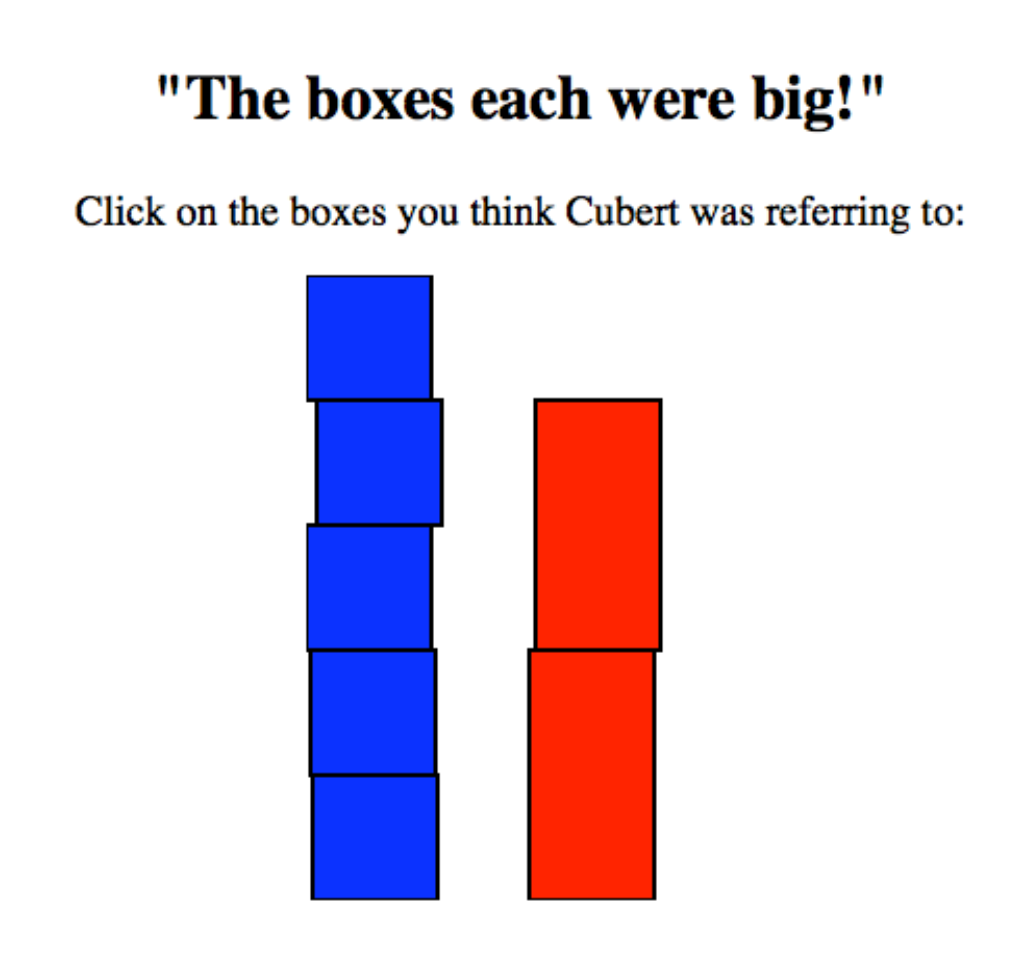
\includegraphics[width=3in]{images/trial2.eps}
	\caption{Example trial from Expt.~1 with the predicate \emph{big} in the ``each'' utterance.}\label{expt1trial}
\end{figure}

Cubert used three predicates, \emph{big}, \emph{heavy}, and \emph{tall}, in three sentence frames, or utterances: ``bare'' \ref{bare}, ``each'' \ref{each}, and ``together'' \ref{together}. Participants saw each version of each predicate in a random order, completing nine trials. All 50 participants indicated that they were native speakers of English, so we included all of the data in the analyses reported below.

\subsection{Predictions}

If \emph{each} and \emph{together} are clear disambiguators for plural predication, we should should find a split in the choice of referent depending on which of these words appears. Encountering distributive \emph{each}, as in \ref{each}, participants should choose the distributive referent (Fig.~\ref{expt1trial}, right); with collective \emph{together}, \ref{together}, participants should choose the collective referent (Fig.~\ref{expt1trial}, left). 

For the potentially ambiguous bare utterances, stubbornly distributive \emph{big} ought to always prefer distributive referents, while complaisantly collective \emph{heavy} should be split. If predicates of size and shape are always stubbornly distributivity, \emph{tall} should pattern with \emph{big}. Given that size and height are visually assessable properties, the scenario manipulation should have no effect on Cubert's epistemic state, and therefore no effect on the resulting interpretations for bare \emph{big} and \emph{tall}. 
%For complaisantly collective \emph{heavy}, we should find higher rates of collective referent choice for the bare utterance. 
However, given that Cubert would need to lift individual boxes to assess their individual weight, we should find an effect of scenario for \emph{heavy}: moving all of the boxes (as opposed to inspecting each box) would yield higher rates of collective referent choice; without lifting each box, Cubert would lack the knowledge needed to be justified in using a distributive interpretation.

\subsection{Results}

Results were coded in terms of whether participants chose the collective referent, and therefore the collective interpretation for Cubert's statement to Dot. Fig.\ \ref{results2} displays the proportion of collective choices, with bootstrapped 95\% confidence intervals drawn from 10,000 samples of the data \citep{diciccioefron1996}; a value of 1 indicates that participants chose the collective referent 100\% of the time.

To evaluate the disambiguating potential of our paraphrases, we first look at responses to these paraphrases, excluding the bare utterance. Mean proportion of collective referent choice for collective paraphrases with \emph{together} was 85\% (i.e., near ceiling); for distributive paraphrases with \emph{each} this proportion was 10\% (i.e., near floor). We fit a mixed effects logistic regression model \citep{baayenetal2008} using the \emph{lme4} package \citep{batesetal2014} in \emph{R}, predicting referent choice by \textsc{utterance} (``each,'' ``together'') and its interaction with \textsc{predicate} (\emph{big}, \emph{heavy}, \emph{tall}; \emph{big} was coded as the reference level), as well as \textsc{trial} order.  The model included random intercepts for participants and scenarios (i.e., the maximal random effects structure supported by the data). The full regression model appears in Appendix \ref{expt1results}. The model finds a main effect of \textsc{utterance} ($\beta$ = 4.99, $SE$ = 0.82, $z$ = 6.08, p $<$ 0.001), confirming that collective \emph{together} yielded greater rates of collective referent choice than distributive \emph{each}; the interactions with \textsc{predicate} were not significant (\emph{heavy}: $\beta$ = -1.39, $SE$ = 0.91, $z$ = -1.52, p $=$ 0.13; \emph{tall}: $\beta$ = -0.63, $SE$ = 0.95, $z$ = -0.66, p $=$ 0.51). The effect of \textsc{trial} was also not significant ($\beta$ = 0.07, $SE$ = 0.07, $z$ = 1.00, p $=$ 0.32). Thus, the ``together'' utterances yielded collective referent choices, and the ``each'' utterances did not, for each of the three predicates.
%\ndg{should we have predicate be a predictor here so that we can report (whether) the predicate didn't affect choice for the fully dissambiguated phrases?}\gcs{if we have predicate interact with utterance, the interaction is not significant. include?}
%\gcs{changed around analysis to include interactions with predicate as predictors}

To evaluate the behavior of the predicates in the absence of the disambiguating particles, together with the effect of our scenario manipulation, we next consider responses to the bare, potentially ambiguous utterance. We fit a mixed effects logistic regression model predicting referent choice by \textsc{predicate} (\emph{big}, \emph{heavy}, \emph{tall}), \textsc{scenario} (``move,'' ``inspect''), and \textsc{trial} order. We dummy coded the \textsc{predicate} predictor, with \emph{big} as the reference level. The model included random intercepts and slopes for participants (grouped by \textsc{trial}; the maximal random effects structure supported by the data). The full regression model appears in Appendix \ref{expt1results}. The model finds main effects of \textsc{predicate} for both the \emph{heavy} ($\beta$ = 3.05, $SE$ = 1.23, $z$ = 2.48, p $<$ 0.05) and the \emph{tall} ($\beta$ = 3.63, $SE$ = 1.29, $z$ = 2.82, p $<$ 0.01) contrasts. Compared to \emph{big}, the other predicates yielded greater rates of collective referent choice in ``bare'' utterances. While the effect of \textsc{scenario} did not reach significance, we note the trend in Fig.~\ref{results2} whereby ``move'' scenarios tended to have higher rates of collective referent choice for bare \emph{heavy} utterances (34\% ``move'' vs.~14\% ``inspect''); a post-hoc test of this difference approaches significance ($t$ = -1.70, \emph{df} = 47.96, $p$ = 0.096).


\begin{figure}[h]
	\centering
	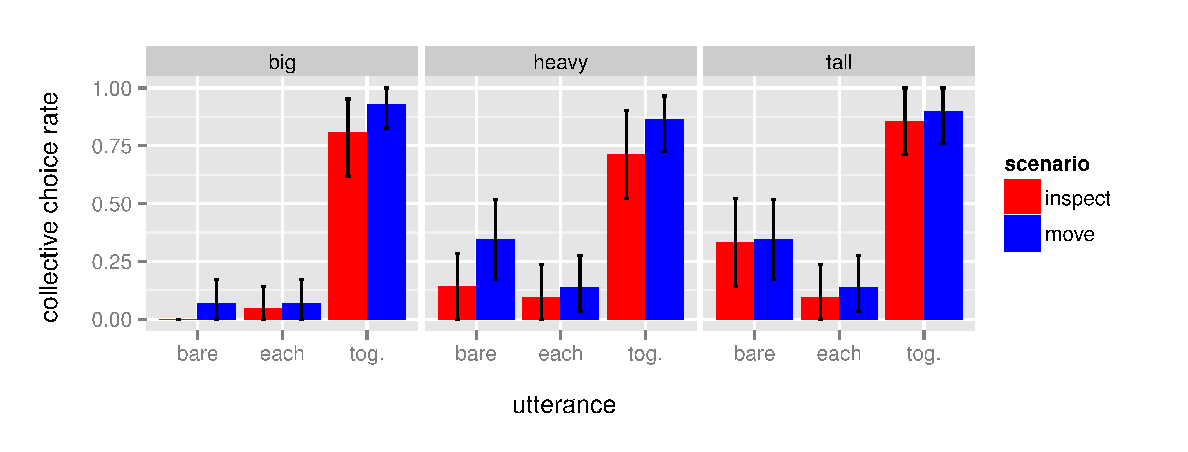
\includegraphics[width=\linewidth]{plots/expt1bootsci.eps}
	\vspace{-15pt}
	\caption{Proportion of collective choices in the results of Expt.~1.}\label{results2}
\end{figure}


\subsection{Discussion}

The disambiguating paraphrases behave as expected: \emph{each} delivers a distributive interpretation and \emph{together} delivers a collective one. We also find that the bare form of \emph{big} patterns differently from \emph{heavy} and \emph{tall}---it is more distributive. This finding is expected with respect to \textit{big} vs.~\textit{heavy} (the former should be stubbornly distributive), but surprising given the behavior of \textit{tall}: both \emph{tall} and \emph{big} are predicates of size and shape. If naming properties of physical extent mediates the choice between distributive and collective interpretations of plural predications, we should find that \emph{tall} patterns with \emph{big}. Equally damning is the comparison between \emph{tall} and \emph{heavy}: if anything, \emph{tall} more consistently delivers collective interpretations. What allows \emph{tall} to readily receive collective interpretations---while precluding them for \emph{big}---in our experimental context? 

As discussed above, one candidate factor is the contextual predictability of the collective property: how easy it is for speakers and listeners to arrive at the same collective property for a given set of objects. We have seen that collective weight is a stable property of sets, which stands to explain the complaisance of \emph{heavy} toward collective interpretations. In the context of the current experiment, collective height is also predictable: boxes  always appeared stacked one on top of the other, yielding stable total set heights. Collective size, however, could vary depending on the strategy used to evaluate it (height? width? area? volume?) as well as on the arrangement of the objects said to hold it, thus accounting for the lack of collective interpretations for bare \emph{big}. In Expt.~3, we use the paraphrase methodology to directly investigate the role of contextual predictability in plural predication.

The results of the current experiment also leave open the possibility of the influence of speaker knowledge in plural predication: based solely on whether the context scenario had Cubert move vs.~inspect the boxes he received, we see a trend whereby bare \emph{heavy} received more or less collective interpretations, respectively. The absence of the effect for \emph{big} and \emph{tall} suggests an explanation in terms of the epistemic state of the speaker: in ``move'' scenarios, the speaker is less likely to have access to individual box weights (having plausibly moved them \emph{en masse}); the listener is therefore less likely to assume that the speaker intended a distributive interpretation for which he lacks evidence. We attempt to confirm this effect with a similar scenario manipulation in Expt.~3.

But before we manipulate contextual predictability and speaker knowledge directly, we extend the paraphrase methodology in Expt.~2 to naturally-occurring examples of plural predication, investigating the role of the local linguistic context.


\section{Experiment 2: Naturally-occurring examples}

In Expt.~1, we used a reference task to validate disambiguating paraphrases as a probe of interpretations of plural predications. 
We next use the paraphrase methodology to evaluate natural plural predications gathered from corpora. We aim to both extend our understanding of distributive vs.~collective preferences to predicates beyond \emph{big}/\emph{tall}/\emph{heavy}, and explore the effect of linguistic context: how the subject noun affects this preference. We thereby test the null hypothesis of a simple lexical distinction between stubbornly distributive and complaisantly collective predicates: if stubbornly distributive predicates are truly stubborn, we should find a clear split in behavior between them and the other predicates, and we should find no effect of the subject noun on their resistance to collective interpretations.
%\ndg{better motivate: we want to see whether there is a clear distinction among predicate classes, we want to see whether noun affects interpretation, etc}

%However, by providing potential referents, we gave participants specific and salient physical arrangements (e.g., box stacks) against which to evaluate interpretations of predicates. Here, we move away from specific arrangements and use the disambiguating paraphrases from Expt.~1 to directly probe interpretations of plural predications.
%We extend beyond big/tall/heavy boxes, to look at frequent linguistic contexts for plural predication. Doing so provides insight into the role the local linguistic context plays in the disambiguation of plural predication.

\subsection{Experiment 2a: Frequent plural predications}

We begin with naturally-occurring examples of plural predications extracted from the British National Corpus.\footnote{Sentences were extracted from the British National Corpus Online service, managed by Oxford University Computing Services on behalf of the BNC Consortium. All rights in the texts cited are reserved.}

\subsubsection{Participants}

We recruited 90 participants through Amazon.com's Mechanical Turk. Participants were compensated for participation.

\subsubsection{Design and methods}

In a search of the British National Corpus, we identified the 40 most frequent subject-predicate combinations in the plural predication frame in \Next.

\ex. The \textsc{noun}s were \textsc{adjective}.

Each participant was presented with 30 sentences; 15 of these sentences were drawn randomly 
%\ndg{was it random?} \gcs{it was random without replacement} 
from the original set of the 40 most frequent instances. The other sentences were constructed by randomly pairing subjects and predicates from the original set of 40 to create 15 novel sentences for each participant. 
%\ndg{were there any restrictions? eg could a participant see the same predicate / subject twice? were the constructed sentences really random for each participant, or was there a fixed set of them?} \gcs{the only restriction was that the sentences were not among the original 40 most frequent ones. a participant could see the same predicate/subject twice in the novel sentences, and they were randomly constructed for each participant}

Each sentence was presented as an utterance by a speaker, and participants were tasked with determining what the speaker meant.\footnote{The full experiment is viewable online at \url{http://cocolab.stanford.edu/experiments/collective/expt2a/expt2a.html}.} Participants rated two possible paraphrases on a sliding scale. The paraphrases were distributive (with ``each'', \ref{bnc-each}) and collective (with ``together'', \ref{bnc-together}). 

\ex. \a. The \textsc{noun}s each were \textsc{adjective}. \label{bnc-each}
\b. The \textsc{noun}s together were \textsc{adjective}. \label{bnc-together}

Given our interest in rates of collective interpretations, we are primarily concerned with collective paraphrase endorsement rates; we expect distributive paraphrase endorsement rates to give redundant information.  We included both distributive and collective paraphrases to highlight the potential ambiguity for participants.
Scale endpoints corresponded to whether the paraphrase was ``definitely'' or ``definitely not'' what the speaker intended by his or her utterance. Before rating its paraphrases, participants judged whether the utterance made sense (choosing between "Yes" and "No"). We analyzed data from the 85 participants who indicated that their native language was English.

%\subsubsection{Predictions}
%
%Our primary goal is to evaluate the viability of our paraphrase methodology with endorsement ratings. If participants understand our task and fully use the sliders to indicate their preferences, we should see a range of paraphrase endorsement ratings. Additionally, if the interpretations of plural predications depend on the immediate linguistic context---that is, on the subjects and predicates involved---we should find by-noun and by-predicate variation in distributive vs.~collective interpretation rates.

\subsubsection{Results}

%\ndg{give some stats on the 'makes sense' judgements: of the original sentences, what was the mean percent sensible? range? for the constructed sentences?}
Of the original 40 most frequent sentences, participants indicated that they ``made sense'' 95\% of the time. Of the novel sentences, participants indicated that they ``made sense'' 67\% of the time.
To avoid possible confusion that nonsensical interpretations might introduce, in the analyses reported below we only look at responses to utterances that participants said made sense. %\ndg{why?}

We begin with a look at the range of collective endorsement ratings.\footnote{A look at distributive endorsement ratings, or normalized collective ratings (i.e., the difference between collective and distributive ratings) reveals similar patterns of results, owing to the high negative correlation between distributive and collective endorsement ratings ($r=-0.78$).} Fig.~\ref{sentence-coll} plots average collective endorsement ratings for each of the 40 most frequent sentences. Descriptively, we see a wide range of ratings, spanning from approximately 25\%  to 85\% endorsement; participants appear to be comfortable using the full scale. An important observation about the distribution of ratings in Fig.~\ref{sentence-coll} is its relatively smooth gradient: we fail to find clear groupings of predicates, such that they behave in one way or another with respect to collective interpretations. Stubbornly distributive \emph{small} indeed occurs toward the low end of collective endorsement ratings, but not markedly so.

\begin{figure}[h!]
	\centering
	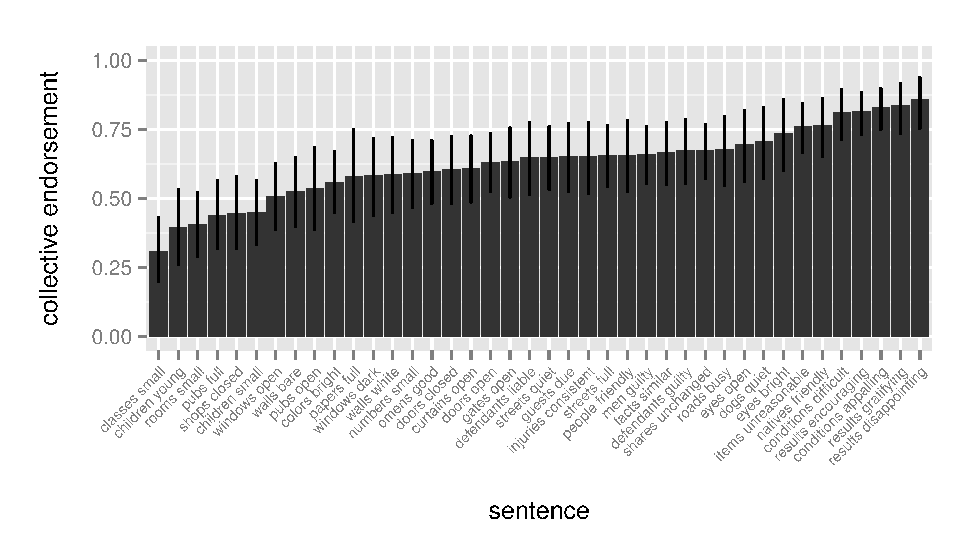
\includegraphics[width=1.04\linewidth]{plots/sentence_plot.eps}
	\vspace{-20pt}
	\caption{Collective paraphrase endorsement rates for different noun-predicate combinations in Expt.~2a (i.e., for different sentences).} \label{sentence-coll}
\end{figure}

There are 8 predicates that occur with multiple nouns in our small corpus; we plot their average collective endorsement ratings in Fig.~\ref{noun-pred-coll}.
%
%
For at least 3 out of these 8 predicates, rates of collective endorsement differ significantly by subject noun (\emph{bright}, \emph{closed}, \emph{small}; see Appendix \ref{2-stats} for details). We draw the reader's attention to the case of stubbornly distributive \emph{small} (bottom right of Fig.~\ref{noun-pred-coll}). 
If stubborn distributivity were a binary, predicate-level phenomenon hard-coded into the semantics, we should find no effect of the subject noun in the determination of \emph{smalls}'s distributive vs.~collective interpretations: stubbornly distributive predicates, regardless of their subject, should always be maximally distributive. But this is not the case for \emph{small} in Fig.~\ref{noun-pred-coll}. 
%More importantly, the subject \emph{numbers} stands out in its relatively high rates of collective endorsement with the predicate \emph{small}. 
A linear mixed effects model predicting collective endorsement rates by subject noun for \emph{small}, with random by-participant intercepts, finds that sentences with the subject \emph{numbers} received greater rates of collective endorsement than sentences with \emph{children} ($\beta=-0.15$, $SE=0.07$, $t=-2.24$, $p<0.05$), \emph{rooms} ($\beta=-0.19$, $SE=0.07$, $t=-2.73$, $p<0.01$), or \emph{classes} ($\beta=-0.27$, $SE=0.07$, $t=-3.87$, $p<0.01$).\footnote{We find the same pattern of results if instead we compare each subject noun with the grand mean (i.e., through effect, or deviation, coding of our variables): \emph{numbers} deviates significantly, while the other nouns do not.} Curiously, \emph{numbers} names objects that do not instantiate physically, which plausibly increases the predictability of their collective size (i.e., their summation) and thus increases rates of collective interpretations.
%\ndg{we should have some analysis of the other seven predicates -- maybe there is an overall test of whether noun matters? or do tests within predicates (add significance stars to the figure...).}\gcs{would it be better to only plot \emph{small} in fig.~\ref{noun-pred-coll}?} 

This analysis relies on the chance occurrence of multiple subject nouns in our small corpora to test the effects of local linguistic context. In Expt.~2b, we follow up on this result by systematically testing the effect of subject nouns on a narrower set of predicates.

\begin{figure}[h!]
	\centering
	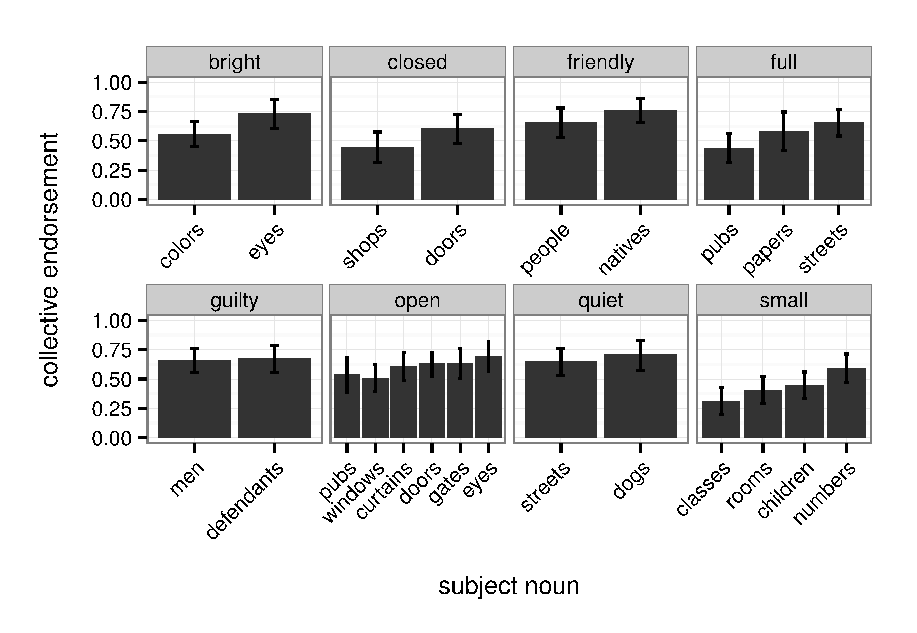
\includegraphics[width=.95\linewidth]{plots/noun_pred_plot.eps}
	%\vspace{0pt}
	\caption{Collective paraphrase endorsement rates for different subject nouns grouped by predicate (Expt.~2a).} \label{noun-pred-coll}
\end{figure}


\subsection{Experiment 2b: \emph{big}, \emph{heavy}, \emph{tall}}

We then narrowed our sights to the predicates tested in Expt.~1: \emph{big}, \emph{heavy}, and \emph{tall}. These predicates are of particular interest because they come from both supposed lexical categories (stubbornly distributive and complaisantly collective) and the physical properties they name lend themselves to direct manipulation.
Due to the limited number of instances of plural predication with these predicates in the British National Corpus, we use instead the much larger Google Books Corpus \citep{davies2011} to look at their most frequent subject nouns.

\subsubsection{Participants}

We recruited 30 participants through Amazon.com's Mechanical Turk. Participants were compensated for participation.

\subsubsection{Design and methods}

The design and methods for this experiment were identical to those of Expt.~2a, with the exception that our naturally-occurring examples feature the predicates \emph{big}, \emph{heavy}, and \emph{tall}, and derive from the Google Books Corpus. We identified the five most frequent subject nouns in the plural predication frame (i.e., \emph{the \textsc{noun}s were \textsc{adjective}}) for each of the predicates \emph{big}, \emph{heavy}, and \emph{tall}.\footnote{For \emph{heavy}, many of the most frequent subject nouns resulted in a non-canonical, abstract interpretation. For example, \emph{heavy rains} or \emph{heavy casualties}. We excluded these cases from the current experiment. In a separate experiment, we included just these abstract instances of plural predication with \emph{heavy} and found no effect of the subject noun on interpretation.} The subject-predicate pairs appear in \Next.

\ex. \emph{Noun-predicate pairings}:\\[2pt]
\begin{tabular}{ll}
	big:& boys, children, houses, rooms, waves\\
	heavy:& bags, lids, loads, men, trees\\
	tall:& buildings, offspring, plants, trees, windows
\end{tabular}	

As with Expt.~2a, participants judged whether the resulting sentences made sense and rated disambiguating paraphrases of each.\footnote{The full experiment is viewable online at \url{http://cocolab.stanford.edu/experiments/collective/expt2b/expt2b.html}.}  We analyzed data from the 26 participants who indicated that their native language was English.

%\subsubsection{Predictions}
%
%\ndg{i don't think we need this section. move any relevant motivation to start of expt....}
%
%Given that \emph{heavy} has been described as complaisantly collective, we should find greater rates of collective interpretation endorsements for this predicate. For stubbornly distributive \emph{big}, we should find much lower rates of collective interpretations. If the relatively high rates of collective interpretations for \emph{tall} in Expt.~1 stemmed from the availability of a specific physical arrangement, we should find lower rates of collective interpretation here, where no arrangements are specified.
%
%If contextual predictability influences the visibility and thus viability of collective interpretations, we should find that noun-predicate pairs that plausibly implicate contextually predictable collective properties---as was the case with \emph{small numbers} in Expt.~2a---yield greater rates of collective interpretations. For example, with \emph{big waves}, the physical instantiation of waves is likely more regular than that of, say, buildings or plants. We might therefore expect greater rates of collective interpretations for \emph{big waves} compared to the other sentences with \emph{big}.
%
%We might also expect to find variation by subject noun that tracks speakers' access to knowledge. That is, if a speaker is more likely to lack evidence for a distributive or a collective interpretation for a specific noun-predicate pair, we should find greater rates of the competing interpretations for that pair. For example, with \emph{heavy loads}, it is unlikely that the speaker carried all of the loads together, so the speaker would lack direct access to knowledge about the collective weight of those loads; we would therefore expect lower rates of collective interpretations as the probability of epistemic access to total, collective weight decreases.

\subsubsection{Results}

Of the original 15 most frequent sentences, participants indicated that they made sense 98\% of the time; of the novel sentences, participants indicated that they made sense 87\% of the time.
We again look only at responses to the original most frequent utterances that participants indicated made sense to them.

%\ndg{here, but also in other expts, should do some analysis of the distributive paraphrase... it's weird to just leave it out. if it is truly redundant with the collective measure, how about quantifying that? ie. report their correlation or such.}

Fig.~\ref{bhtcoll} plots average collective endorsement ratings for each of the three predicates grouped by their subjects.\footnote{As in Expt.~2a, distributive endorsement ratings provide redundant information, owing to their high negative correlation with the collective ratings ($r=-.98$).}
%
%
To compare the predicates with each other, we fit a linear mixed effects model predicting collective endorsement by predicate, with random intercepts for participants and nouns, and random slopes for participants. The predicate predictor was dummy coded with \emph{heavy} as the reference level. There were main effects for both contrasts, such that \emph{big} ($\beta=-0.22$, $SE=0.07$, $t=-3.24$, $p<0.01$) and \emph{tall} ($\beta=-0.20$, $SE=0.06$, $t=-3.20$, $p<0.01$) led to lower rates of collective endorsement than \emph{heavy}. 

We might take the split in behavior between \emph{heavy} on the one hand and \emph{big} and \emph{tall} on the other as evidence for a categorical divide between complaisantly collective and stubbornly distributive predicates. However, comparing the predicates at the level of individual subject nouns suggests otherwise: the subject noun with the highest rates of collective endorsement for \emph{big}, \emph{waves}, yields rates of collective endorsement that do not differ significantly from \emph{heavy}'s least collective subject noun, \emph{men} (42\% \emph{big waves} vs.~38\% \emph{heavy men}; $\beta=-0.04$, $SE=0.09$, $t=-0.51$, $p=0.62$). The same holds of the comparison between \emph{tall}'s most collective subject noun, \emph{trees}, and \emph{heavy men} (30\% \emph{tall trees}; $\beta=-0.07$, $SE=0.08$, $t=-0.87$, $p=0.39$). 


\begin{figure}[htb]
	\centering
	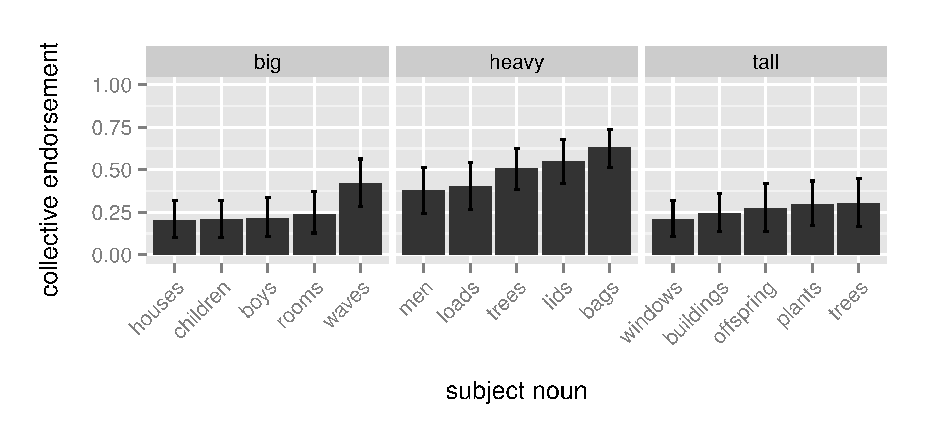
\includegraphics[width=.85\linewidth]{plots/bht_plot.eps}
	\vspace{0pt}
	\caption{Collective paraphrase endorsement rates for different nouns serving as the subject to the predicates \emph{big}, \emph{heavy}, and \emph{tall} (Expt.~2b).} \label{bhtcoll}
\end{figure}

%\ndg{it's not clear to me that the ensuing are the most useful analyses to do... we want to know how judgements vary by noun. it is relevant to know if any nouns differ within predicate, and also whether the ranges of the predicates overlap....}

Next, we compare the behavior of the subject nouns within each predicate.  Starting with \emph{tall}, we fit a linear mixed effects model predicting collective endorsement by subject noun, with random intercepts for participants; full regression models appear in Appendix \ref{2-stats}. The subject noun predictor was dummy coded with \emph{trees} as the reference level (i.e., the subject with the highest average collective endorsement rating). Compared to \emph{trees}, we do not find an effect of the contrast with \emph{plants} ($\beta=0.00$, $SE=0.06$, $t=-0.07$, $p=0.95$), \emph{offspring} ($\beta=-0.03$, $SE=0.06$, $t=-0.55$, $p=0.59$), \emph{buildings} ($\beta=-0.06$, $SE=0.06$, $t=-1.00$, $p=0.32$), or \emph{windows} ($\beta=-0.09$, $SE=0.06$, $t=-1.52$, $p=0.13$). In other words, \emph{tall}'s subjects behave similarly in their general resistance to collective interpretation. 

Turning to \emph{big}, we performed a similar analysis, this time dummy coding \emph{waves} (the subject with the greatest average collective endorsement rating) as the reference level. There were significant effects of each contrast: \emph{rooms} ($\beta=-0.18$, $SE=0.06$, $t=-2.97$, $p<0.01$), \emph{boys} ($\beta=-0.22$, $SE=0.06$, $t=-3.53$, $p<0.01$), \emph{children} ($\beta=-0.21$, $SE=0.06$, $t=-3.54$, $p<0.01$), and \emph{houses} ($\beta=-0.23$, $SE=0.06$, $t=-3.68$, $p<0.01$); \emph{waves} stands out in its relatively high levels of collective endorsement with \emph{big}.

Finally, \emph{heavy}; here, \emph{bags} received the highest collective endorsement ratings, so we coded it as the reference level. The contrast with \emph{lids} was not significant ($\beta=-0.08$, $SE=0.08$, $t=-1.04$, $p=0.30$), the contrast with \emph{trees} was marginally significant ($\beta=-0.15$, $SE=0.08$, $t=-1.93$, $p=0.06$), and the contrasts with \emph{loads} ($\beta=-0.24$, $SE=0.08$, $t=-3.15$, $p<0.01$) and \emph{men} ($\beta=-0.25$, $SE=0.08$, $t=-3.56$, $p<0.01$) were significant. In other words, we find similarly high ratings for \emph{bags} and \emph{lids}, intermediate ratings for \emph{trees}, and similarly low ratings for \emph{loads} and \emph{men}.

\subsubsection{Discussion}

\ndg{to edit...}

We have extended our paraphrase methodology beyond a simple reference task, using naturally-occurring examples of plural predications.
% Our goals here were modest: to understand better the terrain of interpretation preferences for plural predications, without special attention to particular classes of predicates or subjects. Participants demonstrated full use of the paraphrase endorsement rating scales provided. Moreover, 
The pattern of ratings sheds some light on the status of stubborn distributivity. Perhaps most striking is the absence of clear groupings of predicates in the results of Expt.~2a: one would be hard-pressed to read stubborn distributivity (or complaisant collectivity) off the gradient of ratings in Fig.~\ref{sentence-coll}.

%The fact that disambiguation preferences differ by subject noun, not only by predicate further shifts the theoretical focus from lexical classes of predicates. If a plural predication can be more or less collective depending on the subject, then we must look at least partly to context in order to understand interpretation preferences.
%After considering the full set of sentences, we narrowed our focus to those predicates occurring in more than one sentence (i.e., with different subject nouns). Narrower still, 

%We highlighted the case of stubbornly distributive \emph{small}, showing that the subject \emph{numbers} yielded higher rates of collective endorsement than other subject nouns. One possible explanation for the exceptional behavior of \emph{numbers} is thus: The collective size of numbers is naturally their sum, 
%Faced with the task of evaluating the relative size of a hypothetical set of numbers, participants converge on a single strategy, namely summing them up. In other words, the collective size of numbers 
%which is relatively predictable in context---more so than the collective size of children (determined by, e.g., height, weight, age, etc.) or of rooms and classes (determined by, e.g., number of occupants, seating capacity, overall volume, etc.). Moreover, numbers do not physically instantiate, so the contextual predictability of their collective size will not suffer from potential variability in their arrangement. 
%We explore this idea further in Expt.~2b, focussing on the theoretically relevant set of predicates: \emph{big}, \emph{heavy}, and \emph{tall}. \ndg{why?}

%\ndg{other discussion begins here}

Narrowing our focus to the predicates \emph{big}, \emph{heavy}, and \emph{tall} in Expt.~2b, we found that complaisantly collective \emph{heavy} indeed does yield greater rates of collective paraphrase endorsement, and that stubbornly distributive \emph{big} and \emph{tall} pattern together in their resistance to collective interpretations. However, once we consider the effect of local linguistic context by comparing responses to specific subject nouns, the division between the two classes of predicates disappears. \emph{Big} and \emph{tall} are no longer so stubborn with the appropriate context (cf.~the relatively high rate of collective interpretations participants demonstrated for \emph{tall} in Expt.~1).

%This finding for \emph{big} aligns with the finding from Expt.~1, where we found a  similar pattern of stubborn distributivity for \emph{big}. For \emph{tall}, however, this finding is at odds with .

%We interpret this finding for \emph{tall} as evidence for the context-dependent nature of these predications. In Expt.~1, participants had specific, salient sets against which to evaluate the property. In the current experiment, this information was lacking, and so were collective interpretations. In other words, without information about how the subject physically instantiates, participants are wary of assigning collective interpretations to predicates of physical extent. Here we again find evidence for the role of contextual predictability of the relevant property in the disambiguation of plural predications: in Expt.~1, collective height was particularly salient (boxes came stacked on top of each other); here, collective height was underspecified (it would depend on the specific physical arrangement of the subject in question).

By comparing specific subject nouns within predicates, we begin to find evidence for the context-dependent nature of these predications. With \emph{big}, four out of the five subject nouns strongly resisted collective interpretations. However, with \emph{waves}, participants much more readily endorsed collective paraphrases. As was the case with \emph{small numbers} in Expt.~2a. Several interpretations of this finding are possible; one is that limiting the noise of a collective interpretation---by reducing the variability in the physical instantiation of the subject---increases the rates of that interpretation. We follow up on this hypothesis with a direct manipulation of predictability in Expt.~3.

%<<<<<<< Updated upstream
Finally, with \emph{heavy}, we found that different subject nouns yielded different rates of collective interpretations. At first blush, these differences appear to track the probability that a speaker would have access to the information necessary to verify a distributive interpretation. Lids and bags are probably picked up together, certainly more so than loads or men. 
If speakers experience only the collective weight of a plurality, not the individual weights of the members, they lack knowledge which would license the distributive meaning. 
If listeners are aware of this, then the alternative, collective reading becomes more likely for collections (such as lids) that are likely to be lifted together.
%Without experiencing the collective weight of a plurality (e.g., of many loads), speakers lack knowledge about whether or not a collective interpretation would be true (e.g., what the total weight of the loads was); without this knowledge, the interpretation becomes less likely, and as a result its alternative, the distributive interpretation, becomes more likely. 
As with contextual predictability, we follow up on this result with a direct manipulation of speaker access to knowledge in Expt.~3.
%=======
%Finally, with \emph{heavy}, we found that different subject nouns yielded different rates of collective interpretations. At first blush, these differences appear to track the probability that a speaker would have access to the information necessary to verify a collective interpretation. Lids and bags are probably picked up together, certainly more so than trees, and yet more so than loads or men. Without experiencing the collective weight of a plurality (e.g., of many loads), speakers lack knowledge about whether or not a collective interpretation would be true (e.g., what the total weight of the loads was); without this knowledge, the interpretation becomes less likely, and as a result its alternative, the distributive interpretation, becomes more likely. As with contextual predictability, we follow up on this result with a direct manipulation of speaker access to knowledge in Expt.~3.
%% NOTE TO SELVES: follow up on this result with two experiments, one extimating object size and another estimating collectivity; then, check the correlation between the two measures
%>>>>>>> Stashed changes


\section{Experiment 3: Manipulating context}

% And with more predictable collective properties, the truth values of statements involving them become more stable, so collective interpretations are less noisy and stand a better chance of being informative. These interpretations should therefore become more likely. 
%If speakers lack knowledge to verify one of two possible interpretations, the epistemically-supported interpretation should become more likely. In Expt.~3, we manipulated predictability and speakers' access to knowledge through a series of context scenarios, and used the paraphrase endorsement method from Expt.~1 to test the availability of collective interpretations.

Physical properties of collections will tend to be more predictable when the physical arrangement is more predictable. 
According to our hypothesis, greater predictability should lead to more collective interpretations.
For instance, if collections of certain boxes are always stacked neatly, the collective height of a stack can be stably predicted (as the sum of individual heights); if these boxes come in jumbled-up piles the collective height is less predictable.
In Expt.~3 we manipulate expectations about the arrangement of boxes, using the paraphrase methodology to test the effect on the interpretation of plural predications. We expect to see an effect on \emph{tall}, whose collective property is the direct target of our manipulation; we also expect to see a more moderate effect on \emph{big} to the extent that big can refer to height; we expect no effect on \emph{heavy}, which is stable regardless of arrangement.

In Expt.~3 we also return to the effect of speaker's knowledge. Recall the prediction of our pragmatic hypothesis, that more collective interpretations should attain when the speaker lacks knowledge about individual object properties (but has knowledge about collective properties). We conjectured that the effect of \emph{heavy}'s subject nouns in Expt.~2 was due to knowledge in this way: for smaller objects the likelihood of interacting with them individually is lower, making the likelihood of individual weight knowledge lower.
In Expt.~1 we attempted to manipulate the likelihood that the speaker had interacted with the boxes individually, via the ``inspect'' scenario, versus only collectively, in the ``move'' scenario. We found a trend in the predicted direction that did not reach significance.
It is possible that this effect was real, but small because of a bias for the distributive referent (leading to a floor effect).
In Expt.~3, we repeat the move/inspect manipulation using the pure paraphrase endorsement dependent measure of Expt.~2, which may have greater sensitivity than a binary choice between possible referents.

%---where ``move'' scenarios dis-privileged distributive knowledge and therefore had greater rates of collective interpretations
%
% ---where collective interpretations appeared to increase as probability of collective knowledge increased
%
%If contextual predictability of collective properties influences the availability of collective interpretations, we should find that regular arrangement contexts yield more collective interpretations, resulting in higher endorsement rates for the collective paraphrase with \emph{together}. This effect ought to hold for the predicates \emph{big} and \emph{tall}---\emph{heavy} is already strongly contextually predictable, so we might not be able to increase its predictability. The predicate \emph{tall} should be the most sensitive to our context manipulation because we introduce regularity into its dimension of measurement directly: stacking boxes on top of each other to make collective height particularly salient.
%
%Given the trending effect of speaker access to knowledge with \emph{heavy} in Expt.~1---where ``move'' scenarios dis-privileged distributive knowledge and therefore had greater rates of collective interpretations---and the significant effect with \emph{heavy}'s subject nouns in Expt.~2---where collective interpretations appeared to increase as probability of collective knowledge increased---we should find a similar effect here: collective paraphrase endorsement for \emph{heavy} should be greater in ``move'' scenarios where distributive knowledge is lacking, independent of the regularity of the context. We have no reason to expect a similar effect for the other two predicates, due to the visual assessability of their corresponding properties, and their insensitivity to the scenario manipulation in Expt.~1.


\subsection{Participants}

We recruited 80 participants through Amazon's Mechanical Turk. Participants were compensated for participation.

\subsection{Design and methods}

The experimental context was similar to that of Expt.~1. Participants were first introduced to an agent, Cubert, who works in a factory with boxes. Cubert receives boxes from a dispenser in the ceiling. Participants began by observing the dispenser in action.\footnote{The full experiment is viewable online at \url{http://cocolab.stanford.edu/experiments/collective/expt3/expt3.html}.} 

Between subjects, we manipulated the \textsc{scenario} story (``move'' vs.~``inspect''): Cubert's job was either to move shipments of boxes, or to inspect them. As in Expt.~1, in ``move'' scenarios, Cubert appeared with a dolly with which to carry the boxes. In ``inspect'' scenarios, Cubert appeared without a dolly.

Also between subjects, we manipulated the variability of the \textsc{context} (``regular'' vs.~``random''). In regular contexts, the dispenser consistently stacked boxes on top of each other (Fig.~\ref{expt2context}, left). In random contexts, boxes were dispensed without any consistent physical arrangement (Fig.\ \ref{expt2context}, right). Participants saw a series of four context priming scenarios; in each scenario, they saw a different set of boxes dispensed.
%\ndg{do the boxes vary at all in the familiarization aside from arrangement? if so describe.}


\begin{figure}[h]
	\centering
	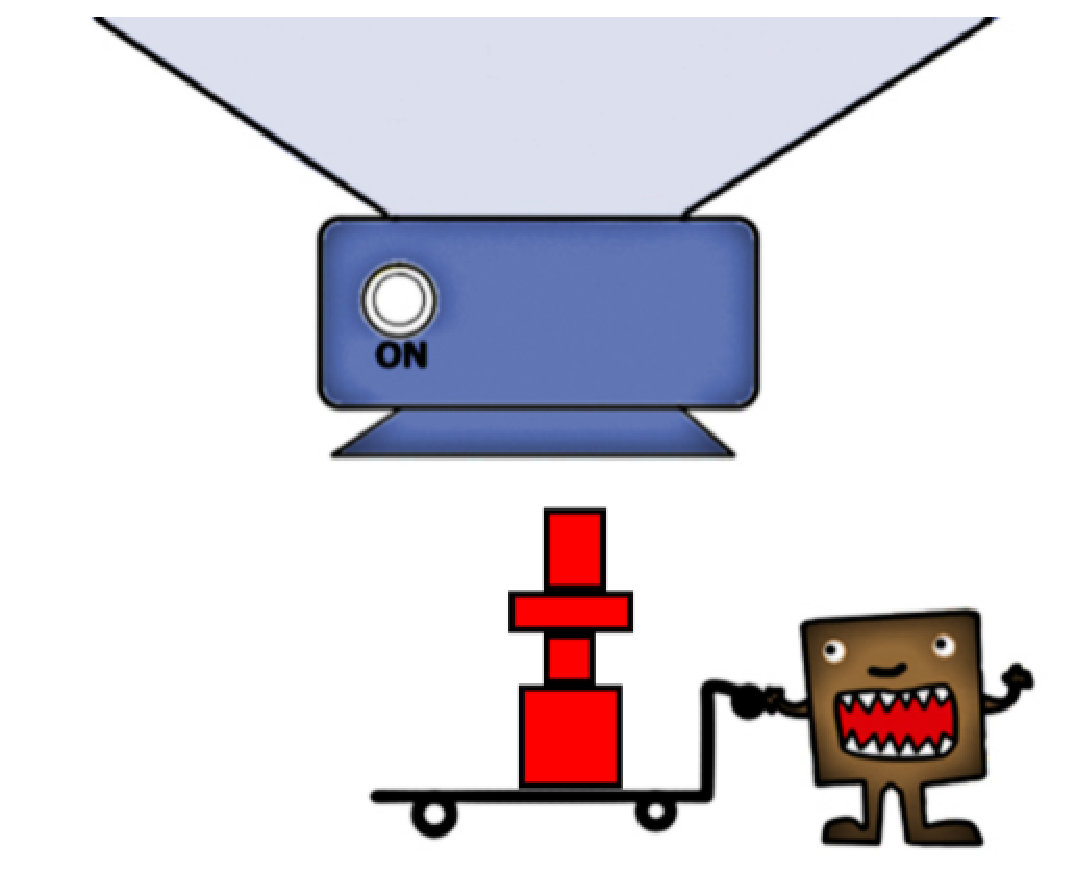
\includegraphics[width=.45\textwidth]{images/context13reg.eps}
	\ \ \ \ 
	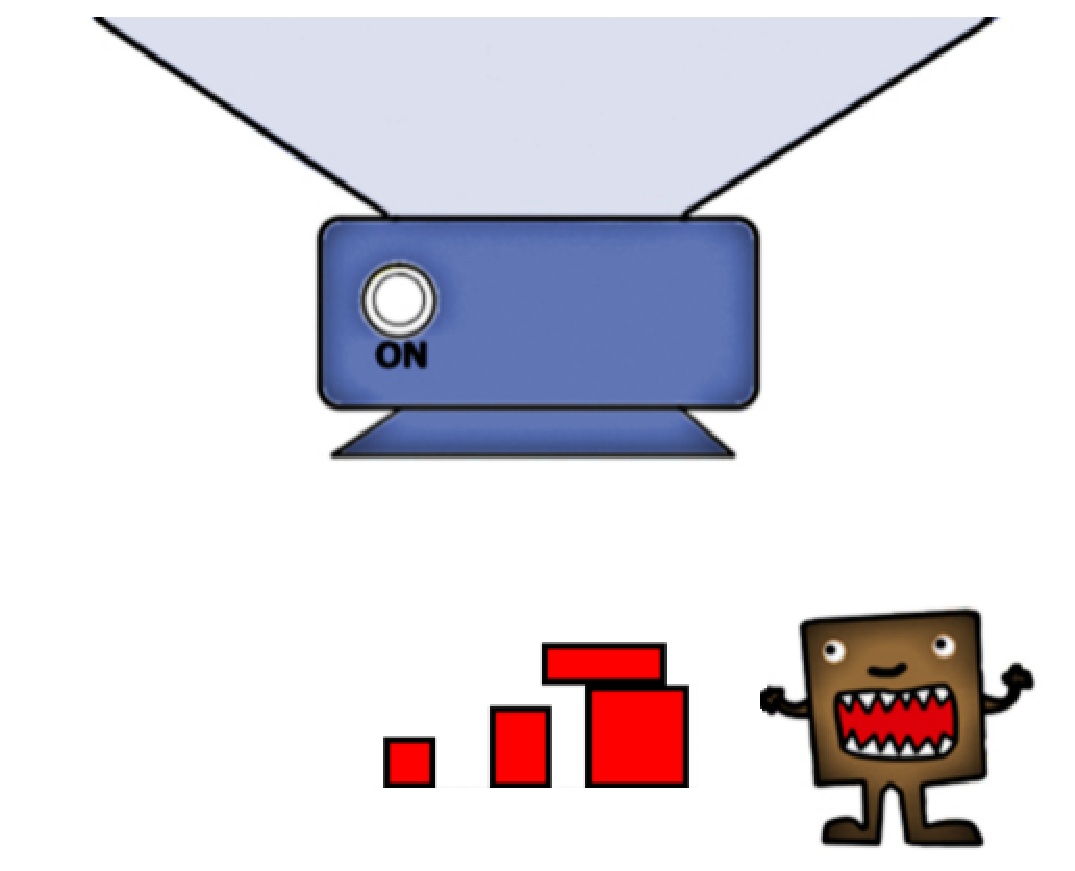
\includegraphics[width=.45\textwidth]{images/context13nodolly.eps}
	\caption{Example context scenarios from Expt.~3. Left: the outcome of a ``regular,'' ``move'' context scenario. Right: the outcome of a ``random,'' ``inspect'' context scenario.\label{expt2context}}
\end{figure}


After observing the dispenser in action via the context  scenarios, participants were then introduced to a second agent, Dot, whom Cubert told about some boxes he moved/inspected. Participants were tasked with helping Dot understand what Cubert meant by his utterance. To do so, they saw an utterance and rated potential paraphrases on a sliding scale (as in Expt.~2). The paraphrases were distributive (with  ``each'') and collective (with ``together'').  Scale endpoints corresponded to whether the paraphrase was ``definitely'' or ``definitely not'' what Cubert meant by his utterance (Fig. \ref{trial}). (Note that, unlike Expt.~1, there was no explicit referent visible.) Participants completed three trials in a random order with three different predicates: \emph{big}, \emph{heavy}, and \emph{tall}. For the analyses reported below, we included data from the 77 participants who indicated that their native language was English.

%\ndg{links to expts? should add for all of them...}

\begin{figure}[h]
	\centering
	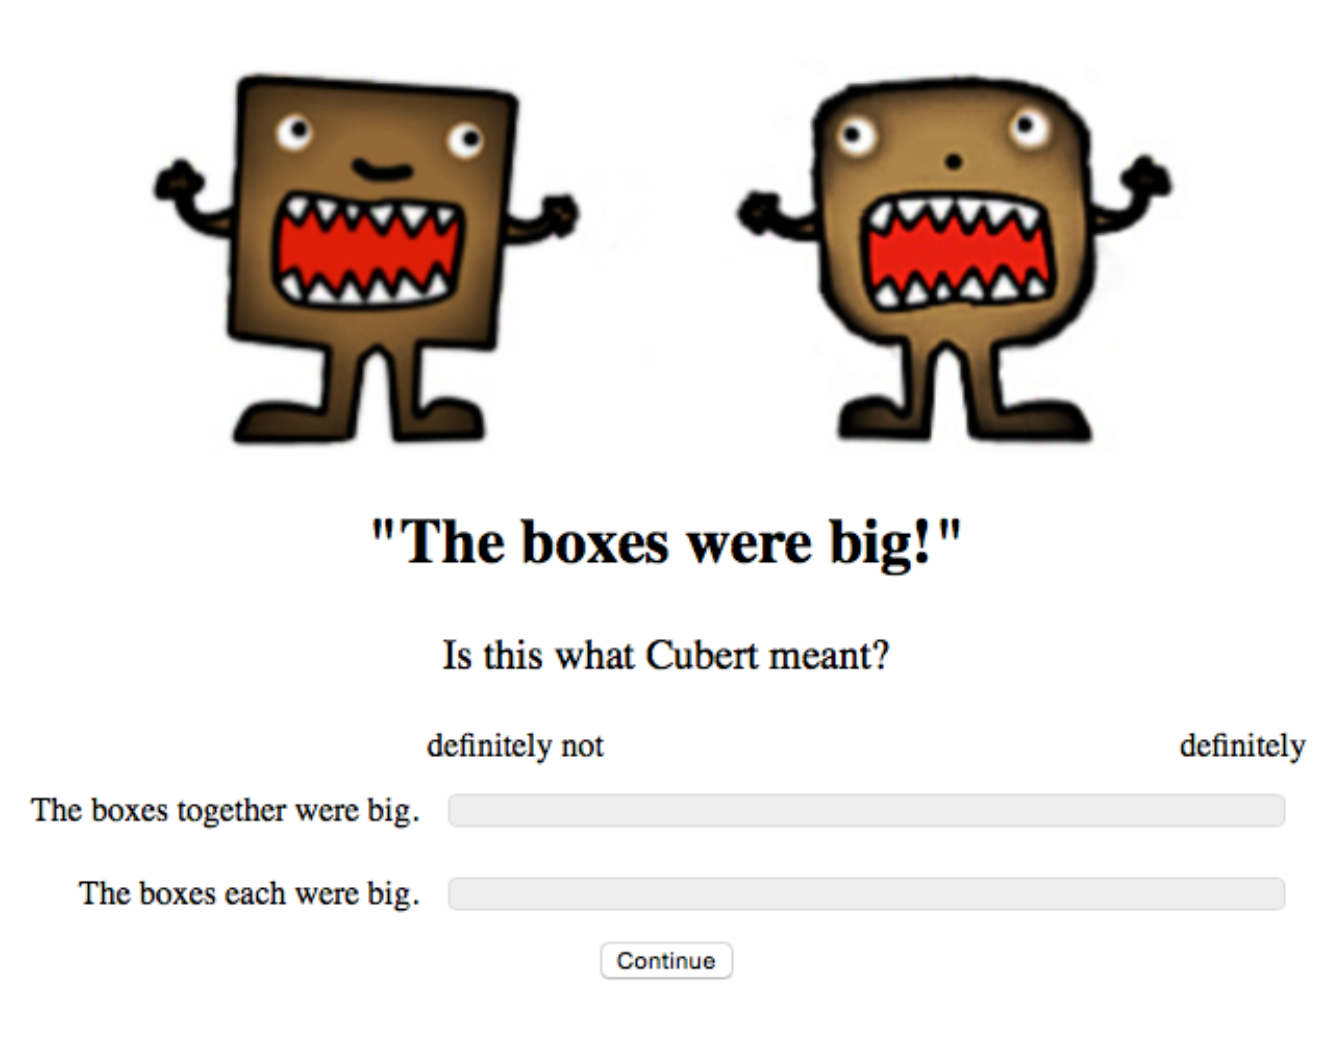
\includegraphics[width=4.5in]{images/trial.eps}
	\caption{Example ``big'' trial.}\label{trial}
\end{figure}

%\subsection{Predictions}
%
%\ndg{i don't think we need this section. relevant motivation can go at beginning of this section. it'll be more compact that way. altermatively, make it shorter and more specific (we predict an interaction between blah and blah, etc).}
%
%If contextual predictability of collective properties influences the availability of collective interpretations, we should find that regular arrangement contexts yield more collective interpretations, resulting in higher endorsement rates for the collective paraphrase with \emph{together}. This effect ought to hold for the predicates \emph{big} and \emph{tall}---\emph{heavy} is already strongly contextually predictable, so we might not be able to increase its predictability. The predicate \emph{tall} should be the most sensitive to our context manipulation because we introduce regularity into its dimension of measurement directly: stacking boxes on top of each other to make collective height particularly salient.
%
%Given the trending effect of speaker access to knowledge with \emph{heavy} in Expt.~1---where ``move'' scenarios dis-privileged distributive knowledge and therefore had greater rates of collective interpretations---and the significant effect with \emph{heavy}'s subject nouns in Expt.~2---where collective interpretations appeared to increase as probability of collective knowledge increased---we should find a similar effect here: collective paraphrase endorsement for \emph{heavy} should be greater in ``move'' scenarios where distributive knowledge is lacking, independent of the regularity of the context. We have no reason to expect a similar effect for the other two predicates, due to the visual assessability of their corresponding properties, and their insensitivity to the scenario manipulation in Expt.~1.

\subsection{Results}

Fig.\ \ref{resultsexpt2} displays the raw paraphrase endorsement ratings averaged across all trials with bootstrapped 95\% confidence intervals. For the purpose of analysis, we analyze responses to the collective paraphrases (i.e., the red bars in Fig.~\ref{resultsexpt2}); higher rates of endorsement for the collective paraphrase signal greater rates of collective interpretation. %calculated the difference between collective and distributive paraphrase endorsement ratings for each trial; Fig.~\ref{normresultsexpt2} presents these difference scores, where greater values of the difference score signal greater rates of collective paraphrase endorsement.
First note the qualitative effects of our two manipulations: collective interpretations do appear to be greater for \emph{tall} and \emph{big} in the ``regular'' conditions, and greater for \emph{heavy} in the ``move'' conditions.

%\ndg{our predictions really are about effect of manipulations on predicates separately, and we don't care much about predicate directly.... so how about doing three separate regressions, one for each predicate? this should be easier to interpret. equivalently we could leave out the main effect predictors for scenario and context, leaving only the interaction terms with predicate. }

\begin{figure}[h!]
	\centering
	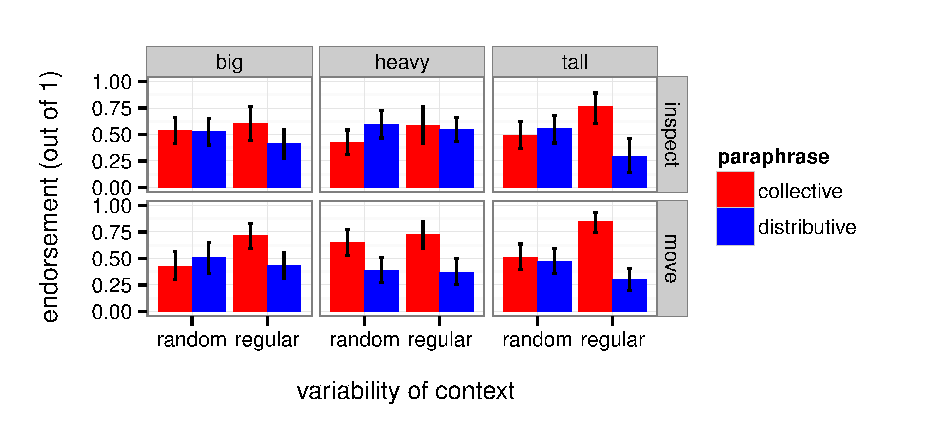
\includegraphics[width=\linewidth]{plots/expt3.eps} 
	\vspace{-20pt}
	\caption{Paraphrase endorsement rate averaged across all trials in Expt.~3.}\label{resultsexpt2}
\end{figure}

For each predicate, we fit a linear regression model predicting collective endorsement ratings by \textsc{context} (``random'' vs.~``regular''),
\textsc{scenario} (``inspect'' vs.~``move''), and \textsc{trial} order; the model also included the interaction between \textsc{context} and \textsc{scenario}.\footnote{All reported results hold if instead we look at normalized collective paraphrase endorsement ratings (i.e., the difference between collective and distributive endorsements for each trial), given the strong negative correlation between the two endorsement ratings ($r=-0.62$). The results also hold if we analyze the results from all three predicates in a single mixed effects regression model; we present the three separate models here for ease of interpretation.} The full regression models appear in Appendix \ref{expt3results}.
As is apparent in Fig.~\ref{resultsexpt2}, there was a main effect of \textsc{context} for both \emph{big} ($\beta$ = 0.18, $SE$ = 0.07, $t$ = 2.52, p $<$ 0.05) and \emph{tall} ($\beta$ = 0.30, $SE$ = 0.07, $t$ = 4.58, p $<$ 0.01), such that regular contexts had more collective interpretations than did random contexts for these predicates. The effect of \textsc{context} was not significant for \emph{heavy} ($\beta$ = 0.11, $SE$ = 0.07, $t$ = 1.43, p $=$ 0.16), but the effect of \textsc{scenario} was ($\beta$ = 0.19, $SE$ = 0.08, $t$ = 2.54, p $<$ 0.05): \emph{heavy} received more collective interpretations in ``move'' scenarios. No other effects reached significance.

%, so that  ($\beta$ = 0.18, $SE$ = 0.07, $t$ = 2.70, p $<$ 0.01). The model finds a main effect of the contrast between \emph{big} and \emph{tall} ($\beta$ = 0.07, $SE$ = 0.04, $t$ = 2.00, p $<$ 0.05), driven in large part by a marginally significant interaction between \emph{tall} and \textsc{context} ($\beta$ = 0.13, $SE$ = 0.08, $t$ = 1.72, p $=$ 0.09): \emph{tall} was most affected by our contextual manipulation, yielding the greatest rates of collective interpretations in regular contexts. Finally, the model finds a significant interaction between the predicate \emph{heavy} and \textsc{scenario} ($\beta$ = 0.21, $SE$ = 0.08, $t$ = 2.77, p $<$ 0.01): 

\subsection{Discussion}

As we would expect if contextual predictability of collective properties influences the viability of collective interpretations, regular contexts had higher ratings for collective paraphrases (and lower ratings for distributive ones). The predicate \textit{tall} was most affected by our contextual manipulation, which directly targeted the height dimension, stacking boxes on top of each other. But \emph{big}, claimed to be stubbornly distributive, is similarly affected: regular contexts yield more collective interpretations. 

For the predicate \emph{heavy}, our contextual predictability manipulation had no measurable effect, presumably because collective weight is already maximally predictable. However, \emph{heavy} was sensitive to the ``move'' vs.~``inspect'' scenario manipulation: as was the trend in the results of Expt.~1, ``move'' scenarios yielded much greater collective endorsement ratings for \emph{heavy}. This manipulation privileges collective interpretations by limiting speakers' access to the information they would need to verify a distributive interpretation; Cubert lacked access to individual box weights in ``move'' scenarios. The predicates \emph{big} and \emph{tall} were not affected by the speaker knowledge scenario manipulation, owing to the fact that they name properties that are visually assessable, and thus visually accessible.

An alternative interpretation of the contextual predictability effect is that in regular, stacked contexts, participants reanalyzed the plural definite description \emph{the boxes} as referring to a single individual (e.g., to a single pile, and not to a set of boxes); if \emph{the boxes} referred to a single individual, there never was any collective predication.
Such a representational coercion story raises serious problems for the semantics of plural definite descriptions \citep[for discussion, see ][]{link1983,landman1989,schwarzschild1996,link1998}. More importantly it is inconsistent with the \emph{lack} of effect for \emph{heavy}: if the pile of boxes was simply represented as an individual when stacked, we would expect greater collective interpretation rates for all predicates in regular contexts.


%An outstanding issue that warrants comment concerns the effect of our contextual predictability manipulation. We identified as regular, high-predictability contexts those in which the box dispenser consistently stacked Cubert's boxes. By regularizing the physical arrangement of the relevant sets, we increased the contextual predictability of the collective properties of physical extent named by \emph{big} and \emph{tall}. This increased contextual predictability led to increased collective paraphrase endorsement. However, one might interpret this result differently: in regular, stacked contexts, participants reanalyzed the plural definite description \emph{the boxes} as referring to a single individual (e.g., to a single pile, and not to a set of boxes). And if \emph{the boxes} referred to a single individual, there never was any collective predication.
%
%In addition to the host of issues such a representational coercion story raises for the semantics of plural definite descriptions \citep[for discussion, see ][]{link1983,landman1989,schwarzschild1996,link1998}, the success of our speaker knowledge manipulation speaks directly against it: participants give similarly high distributive endorsement ratings for \emph{heavy} in ``inspect'' scenarios and similarly low distributive endorsement ratings for \emph{heavy} in ``move'' scenarios, regardless of the variability of context. In other words, the speaker knowledge manipulation, which suppresses information about individual set members in ``move'' scenarios, affects random and regular contexts similarly. If regular contexts forced reanalysis of \emph{the boxes} as an assemblage like \emph{the pile}, we would not expect ``move'' vs.~``inspect'' scenarios to privilege or dis-privilege access to information about individual set members; there would only be a single individual available in context.

Taken together, our results demonstrate the central role of context in plural predication: as collective properties become more predictable, collective interpretations become more likely; and without epistemic support, distributive interpretations become less likely. These findings support a pragmatic account of stubborn distributivity according to which ostensibly stubbornly distributive predicates are such because the properties they name are unpredictable, or unstable in most contexts. We next formalize the role of context in the interpretation of plural predication, using tools from probabilistic modeling.

%Next, we formalize the role of context in this choice of interpretation using a Bayesian Rational Speech-Act model \citep{frankgoodman2012,lassitergoodman2013}. Noisy (i.e., more variable) interpretations are less useful because they require more coordination between speakers and listeners; they are therefore less likely. Similarly, listeners are less likely to assume interpretations for which speakers lack knowledge.



\section{Modeling plural predication}
\label{model}

%\ndg{this section should be much shorter -- probably about three pages. 
%%
%first describe the basic model structure briefly, giving some intuition and pointing out where we draw on previous modeling work.
%%
%start with the literal semantics: $\sem{u}^{v,c}(s)$, which is a truth function that depends on both context, $c$, and utterance interpretation, $v$. specifically we assume that depending on $v$ the plural predication is either universal of property or c X sum of property. here context c is a simple scalar multiplier, a simple approximation for all the ways context could affect the collective property.
%%
%now the literal listener has prior uncertainty about context $P(c)$ and state $P(s)$ and otherwise just updates beliefs by conditioning on the meaning. we could have the literal listener reason also about the word-sense, $v$, but we choose instead to \emph{lift} it, so that pragmatic forces will affect it. (should we implement and compare to the unlifted model?)
%%
%then the speaker, whose utility is expected informativity. (do we need cost in this model?)
%then the pragmatic listener, who reasons about word-sense as well as world (and context).
%%
%then have a briefer section on the setup we use for the boxes scenario, and how we choose parameters.}

We aim to formalize the pragmatic account described so far, especially the role contextual predictability and speaker knowledge in ambiguity resolution.
We will base our analysis on the Rational Speech-Acts (RSA) approach \citep{frankgoodman2012,goodmanstuhlmuller2013}. Within the RSA framework, language understanding is modeled as a social reasoning process: the listener interprets an utterance by reasoning about a cooperative speaker who is trying to inform a naive listener about some state of affairs. 

%Using Bayesian inference, the listener determines what the state of the world is likely to be given that a speaker produced some utterance, knowing that the speaker is reasoning about how a listener is most likely to interpret that utterance. Thus, we have at least three levels of inference. At the top, the sophisticated, pragmatic listener, \emph{L}$_{1}$, reasons about the pragmatic speaker, \emph{S}$_{1}$, and infers the state of the world \emph{s} given that the speaker chose to produce the utterance \emph{u}. The speaker chooses \emph{u} by maximizing the probability that a naive, literal listener, \emph{L}$_{0}$, would correctly infer the state of the world \emph{s} given the literal meaning of \emph{u}.

In several recent RSA models, the pragmatic listener is extended to reason over factors needed to fix meaning, in addition to the sentence itself. 
That is, some aspect of the literal interpretation model is ``lifted'' into the inference performed by the \gcs{pragmatic?}parhatic reasoner.
%In recent models, conversational participants reason not merely over utterances and meanings, but also over variables that contribute to those meanings. 
This sort of lifted variable RSA model has proven useful in accounts of gradable adjective semantics (where the lifted variable is the adjective's degree threshold; \citealp{lassitergoodman2013}), specificity implicatures (where the lifted variable determines the choice of lexica; \citealp{bergenetal2012}), and non-literal meaning (where the lifted variable concerns the dimension along which the speaker intends to communicate, or the question under discussion; \citealp{kaoetal2014}), to name a few applications (see also \citealp{goodmanlassiter2015} for an overview). Our model treats the two underlying senses (collective and distributive) as vague expressions that have an underspecified threshold semantics---following \citealp{lassitergoodman2013}, we lift the corresponding threshold variables to be resolved by the pragmatic listener.

From \citealp{goodmanstuhlmuller2013}, we borrow a treatment of the speaker's knowledge. The speaker has a basic motivation to inform the listener about the true state of the world; he accounts for his uncertainty about this true state by choosing an utterance according to the \emph{expected informativity} given his belief distribution. The pragmatic listener knows this, but does not know what private observations the speaker has had---she takes this uncertainty into account when evaluating an utterance.

There are two significant innovations in the current model. First, we treat ambiguity resolution via a lifted variable: the pragmatic reasoner infers which sense (collective or distributive) of the plural predication was intended by the speaker. Second, we explore the effects of contextual noise that differentially affects the two interpretations. That is, we allow that there are uncertain contextual factors that affect evaluation of the collective property but not the distributive. 
In the formal exposition that follows, we will be brief about the pre-existing model features (lifted threshold variables, speaker knowledgeability) and more expansive about the new aspects.

\subsection{The model}

We take states of the world, $s\in S$, to consist of a collection of entities, each of which has some individual degree: for each $x\in s$, $d(s)\in \mathbb R$ is the relevant property.
We assume a simple truth-functional literal semantics, wherein a plural predication utterance $u$ (e.g., \emph{the boxes are big})  denotes a mapping from states of the world to truth values.\footnote{We assume truth values are coerced to numbers where appropriate: \emph{true} is $1$ and \emph{false} is $0$.} We parameterize the truth function, $\sem{u}^{v,c,\theta_c,\theta_d}: S \rightarrow \text{Bool}$, so that it depends both on context, $c$, and on utterance interpretation, $v$, and two gradable thresholds, $\theta_c$ and $\theta_d$. 
We will consider three alternative utterances: 
an {unambiguously distributive} (e.g., \emph{the boxes each are big}), an {unambiguously collective} (e.g., \emph{the boxes together are big}), and an {ambiguous} utterance (e.g., \emph{the boxes are big}).

\ex. \emph{Literal semantics}:
\a. \label{dist}\sem{\texttt{distrib}}$^{\theta_d}$ = 
\lam $s$. $\forall \ x\ \in s\ [d(x) > \theta_d]$
\b. \label{coll}\sem{\texttt{coll}}$^{c,\theta_c}$ = 
\lam $s$. $[c + \sum_{x\in s} d(x) > \theta_c]$
\c.  \label{amb}\sem{\texttt{amb}}$^{v, c, \theta_d, \theta_c}$ = 
if $v$ \sem{\texttt{distrib}}$^{\theta_d}$, else \sem{\texttt{coll}}$^{c,\theta_c}$

The unambiguous distributive utterance, \Last[a], is a universal quantification over a vague scalar meaning: each object's degree must exceed the distributive threshold $\theta_d$. 
The unambiguous collective utterance, \Last[b], is again a vague scalar meaning: the collective degree must exceed the collective threshold $\theta_c$. 
However, the collective degree captures two assumptions. First, we follow the work on collective semantics in assuming that the appropriate aggregation is based on a sum \citep[e.g.][]{scha1984}: the total degree of the collection.
Second, we assume that the computation of this total degree may depend on contextual factors $c$ (such as the particular arrangement of the objects); we treat $c$ as a simple additive variable that can distort the total degree of the state---an approximation of the many ways that context could affect the collective property. 
Finally, the ambiguous utterance, \Last[c], is governed by the variable $v$: depending on $v$ it is either collective or distributive.

%Specifically, we assume that, depending on $v$, the plural predication is either interpreted distributively, \Next[a], or collectively, \Next[b]. Each of these senses may further depend on context, $c$.
%
% \ex. \emph{Literal semantics}:
% \a. \label{dist}\sem{\texttt{distributive-interpretation}} =
%\begin{flushright}\lam $s$. $\forall \ x\ \in s\ [d(x) > \texttt{distributive-threshold}]$\end{flushright}
%\b. \label{coll}\sem{\texttt{collective-interpretation}}$^{c}$ = 
%\begin{flushright}\lam $s$. $[c \cdot \sum_{x\in s} d(x) > \texttt{collective-threshold}]$\end{flushright}
%
%We are interested in the contextual factors that affect only the collective interpretation, since these lead to differential predictability of the meaning.
%We further make the simplifying assumption that the collective property is formed by summing the individual degrees in a way that may be influenced by context; we treat $c$ as a simple scalar multiplier that can distort the total degree of the collection---an approximation of the many ways that context could affect the collective property. 
%%As $c$ increases, the listener's estimate of the collective property deviates from the true value; more extreme values for $c$ lead to noisier collective interpretations. \ndg{this last sentence isn't right if $c$ is a detemerministic multiplier -- i think this refers to the distribution on $c$...}


The literal listener $L_{0}$ has prior uncertainty about the context, $P(c)$, and the true state, $P(s)$, and otherwise updates beliefs about $s$ by conditioning on the meaning of $u$: 
$$P_{L_{0}}(s|u,v,\theta_d,\theta_c) \propto \sem{u}^{v,c,\theta_d,\theta_c}(s) \cdot P(c) \cdot P(s)$$
The distribution on collective-context, $P(c)$, will determine how predictable the collective property is compared to the distributive: higher entropy $P(c)$ will correspond to noisier collective interpretations.
The other interpretation variables ($v$, $\theta_d$, $\theta_c$) are lifted, so that they will be actively reasoned about by the pragmatic listener. Put simply, the pragmatic listener resolves the interpretation of an ambiguous utterance and fixes the appropriate thresholds for vague gradable predicates.
\ndg{should we say a word about why we choose to lift some but not all of the variables? what happens if we lift $c$???} \gcs{I wonder if it's worth getting into this here..}
%We could have the literal listener reason also about the utterance interpretation, $v$, but we choose instead to \emph{lift} it, so that pragmatic forces will affect it. 

The speaker, $S_{1}$, chooses an utterance \emph{u} that would most effectively communicate some state \emph{s} to a literal listener \emph{L}$_{0}$.  In other words, the speaker's utility function $U_{S_{1}}$ minimizes the effort \emph{L}$_{0}$ would need to arrive at \emph{s} from \emph{u} (i.e., increasing utterance informativity by decreasing surprisal), all while being efficient at communicating (i.e., minimizing utterance cost, $C(u)$):
$$U_{S_{1}}(u;s,v,\theta_d,\theta_c) = \textrm{log}(L_{0}(s|u,v,\theta_d,\theta_c)) - C(u)$$
To capture the speaker's epistemic state, we follow \cite{goodmanstuhlmuller2013} by assuming the speaker has a private belief distribution about the state of the world, $P(s|o)$, that depends on some observations $o$ of the true world. 
The speaker then selects an utterance $u$ to convey information about the likely state $s$ that generated the observation $o$:
$$P_{S_{1}} (u|o,v,\theta_d,\theta_c) \propto \textrm{exp}(\alpha \mathbb{E}_{P_a(s|o)}[U_{S_{1}} (u;s,v,\theta_d,\theta_c)])$$
We will assume, based on our experimental setup, that the speaker has one of two modes of \emph{access} to the world state: if $a=\texttt{full}$, then the speaker has observed the full state, in which case $P_{\texttt{full}}(s|o) = \delta_{s=o}$ is a delta distribution on the true (observed) state; if $a=\texttt{sum}$, then the speaker has only observed the sum (e.g., observing the total weight of some boxes by lifting them together), in which case the speaker considers all of the possible states that could have led to the sum observation, $P_{\texttt{sum}}(s|o)\propto P(s)\delta_{\sum_{x\in s} d(x) = o}$.

%may have observed 
%
%The observations $o$ could be the full state (degree of all objects in $s$) could be a partial state (degree of some of the objects) or could be a value derived from the state---for our purposes an observation of only the total, $\sum_{x\in s} d(x)$, will be relevant. $P(s|o)$ is formed by bayesian updating given the observation.


At the top level of inference, the pragmatic listener $L_{1}$ interprets the speaker's utterance $u$ to jointly infer the state $s$ and
the free interpretation variables: the ambiguous utterance's intended interpretation $v$, and the thresholds $\theta_d$, $\theta_c$. %This probability is proportional to the probability that $S_{1}$ would choose to utter $u$ with interpretation $v$ to communicate about the state \emph{s} inferred on the basis of perceptual access $a$ to a literal listener, while incorporating prior uncertainty about $s$ and $v$.
By Bayes' rule:
$$P_{L_{1}}(s,v,\theta_d,\theta_c|u,a) \propto P_{S_{1}}(u|o(a,s),v,\theta_d,\theta_c) \cdot P(s) \cdot P(v) \cdot P(\theta_d,\theta_c)$$
Here $o(a,s)$ is a deterministic function that reads off the observation the speaker would have had given an access mode and a hypothesized true state.

The plural predication is both ambiguous ($v$) and vague ($\theta_{c}$, $\theta_d$); the listener reasons about likely interpretations given an intuitive understanding of speakers and prior knowledge of the world (i.e., which states and interpretations are \emph{a priori} likely). This inference is guided by reasoning about how informative each utterance would have been, with different interpretations. Informativity is in turn influenced by semantic factors including the variability of context, $c$, that may differentially affect the different interpretations.


%For example, if the speaker only has perceptual access to the sum of some state (e.g., total weight), the speaker would infer a distribution over the possible individual properties that could have generated that observation (e.g., the weights of individual boxes). The speaker thus selects an utterance $u$ to convey information about the likely state $s$ that generated the observation $o$. The revised  pragmatic speaker model, \Next, takes into account perceptual access and potential uncertainty about the world state. Here, the pragmatic speaker calculates a belief distribution over what the actual state $s$ would be given the observation $o$ and perceptual access $a$: $P(s|o,a)$.
%
%
%
%
%
%This trade-off between efficacy and efficiency is not trivial: speakers could always use minimal ambiguity, but unambiguous utterances tend toward the unwieldy, and, very often, unnecessary.
%
%We have seen that disambiguating plural predication depends not only on local linguistic context (e.g., the predicate, its subject, and disambiguating particles like \emph{each} or \emph{together}), but also on the broader discourse and world context. Moreover, we showed how properties of the broader context stand to explain the effect certain predicates have on disambiguating plural predication: complaisantly collective predicates like \emph{heavy} name collective properties that are stable and predictable on the basis of context; stubbornly distributive predicates like \emph{big} name collective properties that are unstable and unpredictable on the basis of context. The less predictable the collective property, the noisier the collective interpretation. Conversely, we saw that increasing contextual predictability increases collective interpretations, presumably by decreasing potential interpretation noise. A noisy interpretation is less useful at communicating its intended message, and therefore less likely. Additionally, we saw that listeners track speaker knowledge as they disambiguate plural predication, so that unsupported interpretations are unlikely. To formalize the effect of context (i.e., contextual predictability and speaker access to knowledge) in plural predication, we adopt a lifted variable variant of the Bayesian Rational Speech-Act model. 
%
%The Rational Speech-Act (RSA) framework views communication as recursive reasoning between a speaker and a listener. The listener interprets the speaker's utterance by reasoning about a cooperative speaker trying to inform a naive listener about some state of affairs. Using Bayesian inference, the listener determines what the state of the world is likely to be given that a speaker produced some utterance, knowing that the speaker is reasoning about how a listener is most likely to interpret that utterance. Thus, we have at least three levels of inference. At the top, the sophisticated, pragmatic listener, \emph{L}$_{1}$, reasons about the pragmatic speaker, \emph{S}$_{1}$, and infers the state of the world \emph{s} given that the speaker chose to produce the utterance \emph{u}. The speaker chooses \emph{u} by maximizing the probability that a naive, literal listener, \emph{L}$_{0}$, would correctly infer the state of the world \emph{s} given the literal meaning of \emph{u}.
%
%In more detail, the pragmatic listener \emph{L}$_{1}$ computes the probability of a state \emph{s} given some utterance \emph{u}. By reasoning about the speaker \emph{S}$_{1}$, this probability is proportional to the probability that \emph{S}$_{1}$ would choose to utter \emph{u} to communicate about the state \emph{s}, together with the prior probability of the state \emph{s}.
%
%\ex. \emph{The pragmatic listener}:\\
%$P_{L_{1}}(s|u) \propto P_{S_{1}}(u|s) \cdot P(s)$
%
%The speaker \emph{S}$_{1}$ desires to choose an utterance \emph{u} that would most effectively communicate some state \emph{s} to a hypothesized literal listener \emph{L}$_{0}$.  In other words, \emph{S}$_{1}$ wants to minimize the effort \emph{L}$_{0}$ would need to arrive at \emph{s} from \emph{u}, all while being efficient at communicating. This trade-off between efficacy and efficiency is not trivial: speakers could always use minimal ambiguity, but unambiguous utterances tend toward the unwieldy, and, very often, unnecessary. \emph{S}$_{1}$ thus seeks to minimize the surprisal of \emph{s} given \emph{u} for the literal listener \emph{L}$_{0}$, while bearing in mind the utterance cost, \emph{C}(\emph{u}). In \Next, we formalize the speaker's utility function \emph{U}$_{S_{1}}$: utterances are more useful at communicating about some state as surprisal and utterance cost decrease.
%
%\ex. \emph{The speaker's utility function}:\\
%$U_{S_{1}}(u;s) = \textrm{log}(L_{0}(s|u)) - C(u)$
%
%%With this utility function in mind, 
%$S_{1}$ computes the probability of an utterance $u$ given some state $s$ in proportion to the speaker's utility function $U_{S_{1}}$. In other words, $S_{1}$ chooses an utterance in proportion to its utility. The term \mbox{$\alpha > 0$} controls the speaker's optimality, that is, the speaker's rationality in choosing utterances. ($\alpha$ corresponds to the temperature parameter of $S_{1}$'s soft-max optimization.)
%
%\ex. \emph{The pragmatic speaker}:\\
%$P_{S_{1}}(u|s) \propto \textrm{exp}(\alpha[\textrm{log}(L_{0}(s|u)) - C(u)])$
%
%At the base of this reasoning, the naive, literal listener $L_{0}$ interprets an utterance according to its meaning. That is, $L_{0}$ computes the probability of $s$ given $u$ according to the semantics of $u$ and the prior probability of $s$. A standard view of the semantic content of an utterance suffices: a mapping from states of the world to truth values.
%
%\ex. \emph{The literal listener}:\\
%$P_{L_{0}}(s|u) \propto \sem{u}(s) \cdot P(s)$
%
%Within the RSA framework, communication is thus modeled as in Fig.~\ref{RSA}, where $L_{1}$ reasons about $S_{1}$'s reasoning about a hypothetical $L_{0}$.
%
%\begin{figure}[h]
%	%\psset{rowsep=20pt,colsep=50pt,nodesep=4pt} 
%	\centering	
%		\psset{arrows=->,rowsep=10pt,colsep=10pt,nodesep=2pt} \begin{psmatrix}
%			\rnode[b]{l1}{$L_{1}$} & \emph{pragmatic listener} & $P_{L_{1}}(s|u) \propto P_{S_{1}}(u|s) \cdot P(s)$\\
%			\rnode[c]{s1}{$S_{1}$} & \emph{pragmatic speaker}
%			& $P_{S_{1}}(u|s) \propto \textrm{exp}(\alpha[\textrm{log}(L_{0}(s|u)) - C(u)])$ \\
%			\rnode[t]{l0}{$L_{0}$} & \emph{literal listener} & $P_{L_{0}}(s|u) \propto \sem{u}(s) \cdot P(s)$
%			\ncline{l1}{s1} 
%			\ncline{s1}{l0} 
%		\end{psmatrix}
%	\caption{Graphical representation of the Bayesian RSA model.}\label{RSA}
%\end{figure}
%
%In its initial formulation, \citet{frankgoodman2012} use the basic RSA framework to model referent choice in efficient communication. To see the mechanism at work, imagine a referential communication game with three objects, as in Fig.~\ref{refgame}. Suppose a speaker wants to signal an object, but only has a single word with which to do so.
%Applying the RSA model schematized in Fig.~\ref{RSA} to the communication scenario in Fig.~\ref{refgame}, the speaker $S_{1}$ chooses a word $u$ to best signal an object $s$ to a literal listener $L_{0}$, who interprets $u$ in proportion to the prior probability of naming objects in the scenario (i.e., to an object's salience, $P(s)$). The pragmatic listener $L_{1}$ reasons about the speaker's reasoning, and interprets $u$ accordingly.  By formalizing the contributions of salience and  efficiency, the RSA framework provides an information-theoretic definition of informativeness in pragmatic inference. This definition will prove crucial in understanding the contribution of contextual predictability of collective properties in the interpretation of plural predication.
%
%\begin{figure}[h]
%	\centering
%	\includegraphics[width=.4\linewidth]{images/communication-game.eps}
%	\caption{Example referential communication scenario from \citet{frankgoodman2012}. Speakers choose a single word, $u$, to signal an object, $s$.}\label{refgame}
%\end{figure}
%
%Continuing with the language game in Fig.~\ref{refgame}, suppose you are the speaker and you want to signal the object in the center to a listener. Your options for $u$ are the words ``blue'' and ``circle''. The clear intuition is to say ``circle,'' and the reasoning behind that intuition readily generalizes: for any utterance you could use, the probability that you pick it to refer to the intended object is inversely proportional to its probability of referring to some other distractor object. We can measure these probabilities for any lexical item in any context, and using the basic RSA model derive quantitative predictions about gradient behavior in human communication. Reason about this reasoning, and you model listener behavior: given that a speaker chose to utter ``circle,'' what object was most likely the intended referent (i.e., the intended meaning)?  %By varying individual features of the objects in visual arrays such as that in Fig.~\ref{refgame}, \citeauthor{frankgoodman2012}
%
%To successfully model ambiguity resolution in plural predication, we need to adopt a variant of the RSA approach wherein speakers and listeners reason not merely over utterances and meanings, but also over variables that contribute to those meanings. This sort of joint-inference ``lifted variable'' (sometimes called ``lexical uncertainty'') RSA model has proven useful in accounts of adjective semantics (where the lifted variable is the adjective's degree threshold; \citealp{lassitergoodman2013}), modal semantics (where the lifted variable is again a threshold, this time for the probability of an event's occurrence; \citealp{lassitergoodman2015}), specificity implicatures (where the lifted variable determines the choice of lexica; \citealp{bergenetal2012}), and non-literal meaning (where the lifted variable concerns the dimension along which the speaker intends to communicate, or the question under discussion; \citealp{kaoetal2014}), to name just a few applications (see also XXX). In our model, the lifted variable about which speakers and listeners reason determines the interpretation of an ambiguous plural predication: whether an utterance is interpreted collectively or distributively.
%
%The ambiguity-resolving free variable $V$ determines the interpretation of a plural predication utterance $u$. When $V$ is \textsc{collective}, $u$ receives a collective interpretation; when $V$ is \textsc{distributive}, $u$ receives a distributive interpretation. Now, the lifted variable literal listener $L_{0}$ computes the probability of some state $s$ given an utterance $u$ and some value for $V$. 
%
%\ex. \emph{The lifted variable literal listener}:\\
%$P_{L_{0}}(s|u,V) \propto \sem{u}^{V}(s) \cdot P(s) \cdot P(V)$
%
%But $L_{0}$ does not know the value of $V$. Put differently, the literal listener does not know the intended interpretation of an ambiguous utterance. The name "lifted variable RSA" captures the fact that this free variable gets passed up from the literal listener through the speaker to be estimated by the pragmatic listener; the pragmatic listener fixes the interpretation by which the literal listener interprets the utterance.
%
%The lifted variable pragmatic speaker $S_{1}$ now incorporates $V$ so that utterances are chosen to best communicate some state $s$ given an interpretation $V$. $S_{1}$ maximizes the likelihood of $u$ given $s$ and $V$, relative to the speaker utility function which minimizes surprisal and the cost of $u$.
%
%\ex. \emph{The lifted variable speaker's utility function}:\\
%$U_{S_{1}}(u;s,V) = \textrm{log}(L_{0}(s|u,V)) - C(u)$
%
%\ex. \emph{The lifted variable pragmatic speaker}:\\
%$P_{S_{1}}(u|s,V) \propto \textrm{exp}(\alpha U_{S_{1}}\!(u;s,V))$
%
%At the top level, the lifted variable pragmatic listener $L_{1}$ interprets an utterance $u$, inferring the state $s$ and resolving the variable $V$. $L_{1}$ now reasons about the speaker, who presumably has an interpretation (i.e., a value for $V$) in mind.
%
%\ex. \emph{The lifted variable pragmatic listener}:\\
%$P_{L_{1}}(s,V|u) \propto P_{S_{1}}(u|s,V) \cdot P(s) \cdot P(V)$
%
%To capture the speaker's epistemic state, our model needs one last element. Following \cite{goodmanstuhlmuller2013}, we include a parameter $a$ determining the speaker's possibly incomplete access to the world state $s$. Now, the speaker makes an observation $o$ about the state $s$, and, depending on the speaker's perceptual access $a$, $o$ might be identical to $s$ (i.e., the speaker has full access to information about the state) or a summary of $s$ (say, its sum, corresponding to the speaker's only having access to the total size or weight of the state). From the observation $o$ and his perceptual access $a$, the speaker generates an expectation about the states $s$ that $o$ might have been an observation of. For example, if the speaker only has perceptual access to the sum of some state (e.g., total weight), the speaker would infer a distribution over the possible individual properties that could have generated that observation (e.g., the weights of individual boxes). The speaker thus selects an utterance $u$ to convey information about the likely state $s$ that generated the observation $o$. The revised  pragmatic speaker model, \Next, takes into account perceptual access and potential uncertainty about the world state. Here, the pragmatic speaker calculates a belief distribution over what the actual state $s$ would be given the observation $o$ and perceptual access $a$: $P(s|o,a)$.
%
%\ex. $P_{S_{1}} (u|o,a,V) \propto \textrm{exp}(\alpha \mathbb{E}_{P(s|o,a)}[U_{S_{1}} (u;s,V)])$
%
%Where speaker's access to knowledge is shared between speakers and listeners (in our experimental setting, participants knew whether Cubert moved the boxes together or inspected each individually), $a$ is shared between $S_{1}$ and $L_{1}$. The full lifted variable RSA model of plural predication appears in Fig.~\ref{pluralRSA}.
%
%\begin{figure}[h]
%	%\psset{rowsep=20pt,colsep=50pt,nodesep=4pt} 
%\centering
%		\psset{arrows=->,rowsep=10pt,colsep=10pt,nodesep=2pt} \begin{psmatrix}
%			\rnode[b]{l1}{$L_{1}$} & \emph{pragmatic listener} & $P_{L_{1}}(s,V|u,a) \propto P_{S_{1}}(u|s,a,V) \cdot P(s) \cdot P(V)$\\
%			\rnode[c]{s1}{$S_{1}$} & \emph{pragmatic speaker} &
%			$P_{S_{1}} (u|o,a,V) \propto \textrm{exp}(\alpha \mathbb{E}_{P(s|o,a)}[U_{S_{1}} (u;s,V)])$ \\
%			\rnode[t]{l0}{$L_{0}$} & \emph{literal listener} & $P_{L_{0}}(s|u,V) \propto \sem{u}^{V}(s) \cdot P(s) \cdot P(V)$
%			\ncline{l1}{s1} 
%			\ncline{s1}{l0} 
%		\end{psmatrix}
%	\caption{The full Bayesian RSA plural predication model. $L_{1}$ infers the state $s$ and an interpretation-resolving variable $V$ given an utterance $u$ and the speaker's perceptual access $a$ to $s$. $S_{1}$ chooses $u$ given an observation $o$ of $s$, certain access $a$ from $o$ to $s$, and an intended interpretation $V$ of $u$. $L_{0}$ infers the state $s$ given some utterance $u$ and its interpretation $V$.} \label{pluralRSA}
%\end{figure}
%
% To summarize: the pragmatic listener resolves ambiguity while interpreting an utterance by reasoning about the pragmatic speaker, who chooses utterances most likely to communicate some state via a specific interpretation to a naive, literal listener. The speaker and pragmatic listener track the speaker's access to knowledge, which determines whether the speaker has limited access to the state about which he communicates. In other words, listeners reason about likely interpretations of ambiguous plural predications given their intuitive understanding of speakers and their prior knowledge of the world (i.e., which states and interpretations are \emph{a priori} likely).

\subsection{Model results}

%\ndg{what is the list of all parameters fit? $P(v)$, $C(u)$... anything else? do these results still use only two values of the degrees (3 and 4)? which $P(c)$ is used for these predictions? is it fit to the data?}

To generate predictions, we need to fix various parameter settings within the model; we aim to make the simplest choices possible, focussing on qualitative predictions.\footnote{The full model is viewable online at \url{http://forestdb.org/models/plural-predication.html}.}
%Here we fill in more details of these settings, with the caveat that the qualitative model results presented below are robust to a broad range of parameter settings; the specific values we give here are used merely to demonstrate the general behavior and success of the model.\footnote{XXX specifics about the range of parameter settings that are possible, and the settings that are not.\label{parameter}}
Each state, $s$, consists of two objects, each of which has degree $3$ or $4$. The prior on states $P(s)$ was taken to be uniform. The distributive threshold $\theta_d$ ranged over the object degrees, and was drawn uniformly from the set of objects; the collective threshold $\theta_c$ ranged over state degrees (i.e., 6, 7 8), and was drawn uniformly from the state prior.
%The priors on state $P(s)$ and on thresholds $P(\theta_d,\theta_c)$ are taken to be uniform. \ndg{check}
We take $P(v)$ to be Bernoulli with a single free parameter (i.e., the prior bias toward collective interpretations); this parameter was fit to $0.9$ based on our experimental data.
We take the cost $C(u)$ to be $1$ for the ambiguous utterance and $2$ for both of the unambiguous utterances---a reasonable assumption from the point of view of production, given that unambiguous utterances contain an extra word (i.e., \emph{each} or \emph{together}). The parameter $\alpha > 0$ controls the speaker's optimality; we fit $\alpha$ to $10$ based on our experimental data.
Importantly, the qualitative patterns reported below are robust to changes in these parameters and assumptions.

%\ndg{what about alpha?}

%States $s$ correspond to ordered sets of four objects, which hold scalar properties. States are formed by drawing four times from a uniform prior distribution over objects (i.e., boxes of size 3 or 4). States are thus sets of positive integers; 
%the state $\{3, 3, 4, 4\}$ corresponds to a plurality of four boxes, two of size 3 and two of size 4. 

%Next, the utterances. Speakers choose between an {unambiguously distributive} (e.g., \emph{the boxes each are big}), an {unambiguously collective} (e.g., \emph{the boxes together are big}), and an {ambiguous} utterance (e.g., \emph{the boxes are big}). The interpretation of the ambiguous utterance depends on the value of the interpretation-resolving variable $v$, which the pragmatic listener infers. When $v$ is \textsc{collective}, the utterance receives a \texttt{collective-interpretation}, \ref{coll}; otherwise, the utterance receives a \texttt{distributive-interpretation}, \ref{dist}.\footnote{Following \cite{lassitergoodman2013}, we treat the threshold parameters as lifted variables that get resolved by the pragmatic listener as he interprets the speaker's utterance. So, strictly speaking, $v$ represents not just the interpretation-resolving variable, but also the threshold variables for the gradable predicates.} %These interpretations carry the semantics in \Next.
% 
% \ex. \emph{Interpretation semantics}:
% \a. \sem{\texttt{distributive-interpretation}} =
%\begin{flushright}\lam $s$. $\forall$x$\in$$s$[x $>$ \texttt{distributive-threshold}]\end{flushright}
%\b. \sem{\texttt{collective-interpretation}} = 
%\begin{flushright}\lam $s$. (\texttt{sum}($s$) $\times$ \textcolor{red}{\texttt{noise}}) $>$ \texttt{collective-threshold}\end{flushright}
%In our box setting, this semantics captures the fact that the distributive interpretation of a gradable predicate is true of a plurality when each of its members exceeds a contextually-determined cutoff \citep{kennedy1999,lassitergoodman2013}. The \texttt{collective-interpretation} is true of a state $s$ just in case the sum of that state---the plurality taken together---exceeds some collective threshold. Here we capture the sum-based aggregation inherent to collective interpretations of gradable predicates \citep{scha1984}. 
%So far, no deviation from the formal semantics tradition.

Our central claim surrounds the effect of $P(c)$, which controls the predictability of the collective interpretation. To evaluate its role, we generated model predictions for distributions of varying entropy; $c$ was drawn from a normal distribution centered around $0$. The variance of this distribution controls the amount of collective interpretation noise. We begin by the comparing effects of \texttt{no} ($\sigma=0.02$), \texttt{low} ($\sigma=1$), \texttt{mid} ($\sigma=2$), and \texttt{high} ($\sigma=3$) collective noise.
%
%What sets this semantics apart is the contextual noise parameter $c$ in the \texttt{collective}-\texttt{interpretation}, a scalar multiplier of the set aggregate estimate that determines contextual predictability. 
%%This parameter explicitly represents possible noise in the determination of, say, collective size. In other words, this parameter models the contextual predictability of a collective property, or the possibility that speakers and listeners will arrive at different truth values for a collective interpretation. For our purposes, lower noise (i.e., values closer to 1) corresponds to increased contextual predictability of the collective property. 
%To evaluate the qualitative predictions of our model, we begin with the possible values for $c$ shown in 
%
%Fig.~\ref{noises} shows four different distributions evaluated. For example, with \texttt{low} noise the multiplier $c$ equals 1 (i.e., no change to the state estimate) 100\% of the time; and with \texttt{high} noise, $c$ equals 0.5, 1, or 1.5 with equal probability (i.e., the state estimate is accurate a third of the time, or off by half two-thirds of the time).
%Given our interest in the effects of contextual predictability and speaker knowledge on the disambiguation of plural predications, i
In Fig.~\ref{modelresults}, we plot the probability that the interpretation-resolving variable $v$ is \texttt{collective} after hearing the \texttt{ambiguous} utterance, marginalizing the other variables from the pragmatic listener $L_1$. In other words, we plot the probability of a collective interpretation depending on collective noise and speaker access.% as a function of noise in the collective interpretation and speaker access to knowledge.

%\begin{figure}[h]
%	\centering
%	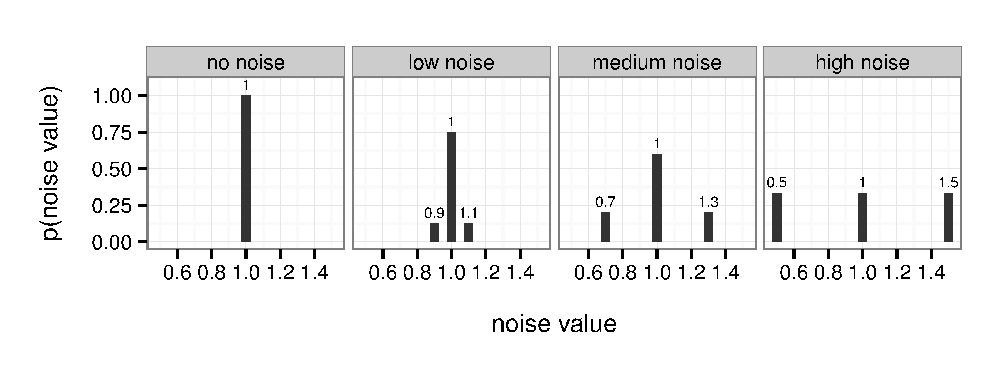
\includegraphics[width=\linewidth]{plots/noise_plots.eps}
%	\vspace{-20pt}
%	\caption{Contextual noise priors used to evaluate the qualitative predictions of the plural predication model.} \label{noises}
%\end{figure}

\begin{figure}[h]
	\centering
	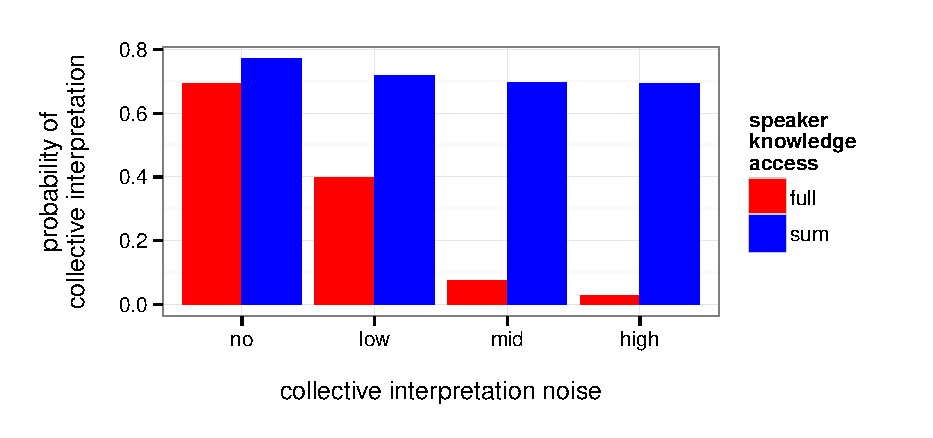
\includegraphics[width=\linewidth]{plots/model-results-add.eps}
	\vspace{-20pt}
	\caption{Model predictions for the probability of the \texttt{ambiguous} utterance receiving a collective interpretation as a function of collective interpretation noise and speaker knowledge access.  
		%\ndg{todo: regenerate this figure using parameters fit to data. also change access label to "sum" from "partial".}  
	} \label{modelresults} 
\end{figure}

%With \texttt{no} noise, our estimates are spot on and collective properties are maximally predictable from context. Increasing noise, contextual predictability decreases: our estimates of collective properties deviate from the true state. Noise is a property of the world context, and as such speakers and listeners both have access to its value. In other words, we assume that speakers and listeners are aware of the inherent contextual predictability of collective properties.

%When the speaker access to knowledge variable $a$ is set to \texttt{full}, the speaker's belief distribution over possible states is exact, a delta distribution over \emph{the} state (Fig.~\ref{speakerbelief}, left); having observed $\{3,3,4,4\}$, the speaker knows the state is $\{3,3,4,4\}$ (and not, say, $\{4,4,3,3\}$). %Where $a$ is set to \texttt{partial} knowledge, the . 
%With \texttt{partial} knowledge, the speaker only observes the sum of the individual state values, say 14, so the speaker's belief distribution is broader (Fig.~\ref{speakerbelief}, right).%But more than one state could generate this value, namely any combination of two size 3 boxes with two size 4 boxes.
%\footnote{In its simplest form, our model includes only objects of two different sizes (3 and 4), so that speaker uncertainty over states concerns the order of the state-internal objects. 
%%Including more possible objects (i.e., more possible object sizes) introduces additional uncertainty over the identity of state-internal objects. 
%We present the simpler model here for illustrative purposes only. All of the model predictions we report are robust to a broad range of parameter settings, including a prior over individual objects that includes more than two possible values. In fact, including more types possible objects serves merely to increase potential speaker uncertainty and thus enhance the effect of speaker knowledge. .}

%\begin{figure}[h]
%	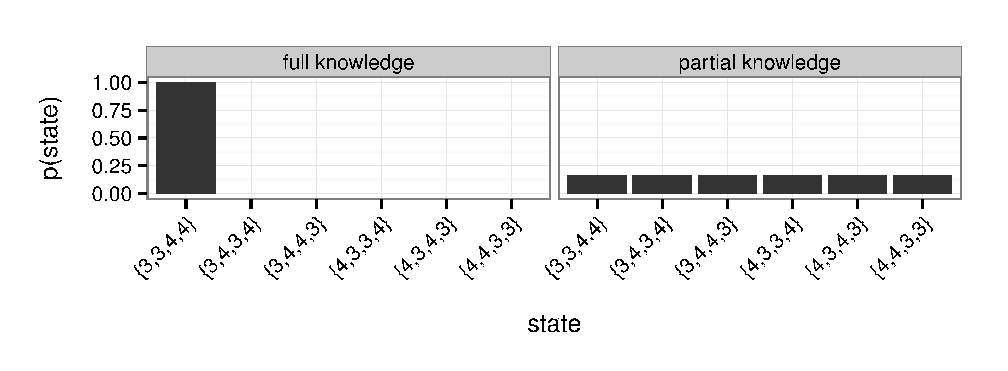
\includegraphics[width=\linewidth]{plots/state_plots.eps}
%	\vspace{-20pt}
%	\caption{Speaker belief distributions resulting from \texttt{full} (left) and \texttt{partial} (right) perceptual access to the state $\{3,3,4,4\}$.} \label{speakerbelief}
%\end{figure}
%%\subsection{Model predictions}


The qualitative predictions of our plural predication model match the hypotheses and experimental results that motivated the model. Most striking is the monotonic decrease in probability of collective interpretations as collective noise increases. We now have a formal understanding as to why this effect holds: the noisier the collective interpretation, the less likely the listener $L_{0}$ is to correctly resolve the question under discussion, namely the properties of the named boxes $s$. Given that the speaker $S_{1}$'s goal is to successfully communicate $s$ to $L_{0}$, the noisier an interpretation, the less useful it is at achieving this goal; the speaker is therefore less likely to intend this interpretation, and as a result the pragmatic listener $L_{1}$ is less likely to infer it.

The model also successfully predicts the qualitative increase in the probability of a collective interpretation when the speaker's  access to individual object properties is limited. %With only partial access to the actual state $s$, $S_{1}$ is less likely to have precise information concerning $s$ about which to communicate. 
$L_{1}$ tracks  $S_{1}$'s epistemic state, and therefore knows whether the speaker has full or partial knowledge. In the case of partial knowledge, a distributive interpretation lacks epistemic support, and therefore becomes less likely; as a result, collective interpretations become more likely.

%We have verified the qualitative predictions of our account of plural predication: increasing the contextual predictability of collective properties (by decreasing contextual noise) increases the probability of collective interpretations; and, regardless of the amount of contextual noise, removing support for a distributive interpretation (by limiting the speaker's access to individual properties) decreases the probability of a distributive interpretation and thus increases the probability of a collective interpretation. Crucially, both of these qualitative predictions are borne out while making minimal assumptions concerning model parameters. Next, we fit these parameters to the human data collected in Expt.~3 to test both qualitative and \emph{quantitative} predictions of the model.


%To test the quantitative predictions of our model, we fit its parameters to best estimate the human data. Comparing the model predictions in Fig.~\ref{modelresults} to the rates of collective endorsement from Expt.~3 in Fig.~\ref{resultsexpt2}, the first thing to notice is the overall higher rates of collective endorsement in the human data. To capture this fact, we can change the prior probability of a collective interpretation, $p(v)$, in our model. In Fig.~\ref{modelresults}, that parameter is set to 0.5, or chance; to achieve a maximal fit between our model and the dependent measure from Expt.~3, we set that parameter to 0.88 for each of the three predicates. We also cheapen the cost of the ambiguous utterance relative to the unambiguous ones; in place of the flat prior distribution over possible utterances used above, here we set the utterance prior such that \texttt{ambiguous} is twice as cheap as \texttt{collective} or \texttt{distributive}---a reasonable assumption from the point of view of production, given that costlier, unambiguous utterances contain an extra word (i.e., \emph{each} or \emph{together}).

%\ndg{something about fitting $P(c)$...}

\ndg{i don't get the next two paragraphs: we're not doing any collapsing here now, right? shouldn't this just read something like ``we fit the variance of $P(c)$ for each predicate and each arrangement condition, we additionally assume total-only knowledge for heavy in move conditions but not other cases. the best fit variance values are blah. the results are compared to expt 3 collective endorsements in fig blah. we see blah.''??}

To quantitatively evaluate the role of speaker knowledge, we collapse over the contextual predictability manipulation and look only at judgments for plural predications with \emph{heavy} (the knowledge manipulation had no measurable affect on \emph{tall} or \emph{big}). %Here we fit only the specific values for noise in the model; all other parameters remain unchanged. 
With \emph{heavy}-specific values for $P(c)$ ($\sigma=0.7$; all other parameters remain unchanged) we generate the model predictions in Fig.~\ref{fit-model}, plotted with average collective endorsement ratings for \emph{heavy} from Expt.~3. By simply assuming that the collective interpretations of \emph{heavy} have \emph{heavy}-specific values for noise in context, we achieve a near exact fit between the model and the human data it predicts.

\begin{figure}[h]
	\centering
	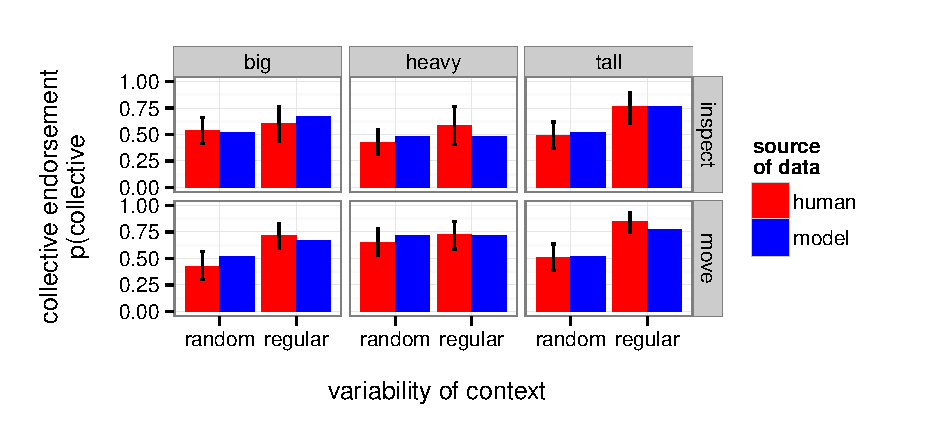
\includegraphics[width=\linewidth]{plots/model_all_new.eps}
	\vspace{-20pt}
	\caption{Fitted model predictions and human data from Expt.~3 for collective interpretations (cf.~Fig.~\ref{resultsexpt2}). For \emph{heavy}, the scenario manipulation (i.e., ``inspect'' vs.~``move'') is modeled by speaker's perceptual access to knowledge of the state (``full'' vs.~``sum''). For \emph{big} and \emph{tall}, variability of context (i.e., ``random'' vs.~``regular'') is modeled by amount of collective interpretation noise $P(c)$.} \label{fit-model}
\end{figure}

To qualitatively evaluate the role of contextual predictability for \emph{big} and \emph{tall}, we again have the model predict collective endorsement, this time collapsing over the scenario manipulation. As with \emph{heavy}, we fit predicate-specific values for $P(c)$; to model the effect of our contextual manipulation, we increased contextual noise in random contexts (\emph{big}/\emph{tall} \texttt{random}: $\sigma=3$; \emph{big} \texttt{regular}: $\sigma=1$; \emph{tall} \texttt{regular}: $\sigma=0.1$).  We also increased the cost of the unambiguous utterances to $3$ (cf.~the cost of $2$ for the results reported above). \ndg{why do we need the costs to vary in this section at all?} With no other changes to model parameters, we generate the predictions plotted in Fig.~\ref{fit-model}; once again, the fit is near perfect.

%\ndg{why not model all of the data, too, uncollapsed? eg i'd like to see a version of fig 9 that has both data and model.... in fact this plus the more qualitative fig 11 may be all we need.}
%
%\begin{figure}[h]
%	\centering
%	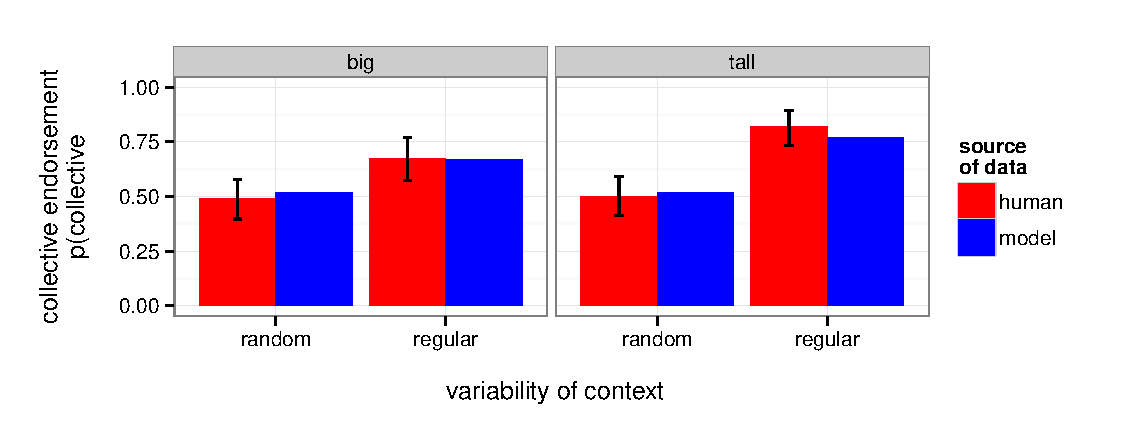
\includegraphics[width=\linewidth]{plots/model-big-tall.eps}
%	\vspace{-20pt}
%	\caption{Fitted model predictions and human data from Expt.~3 for collective interpretations of \emph{big} and \emph{tall}; variability of context (i.e., ``random'' vs.~``regular'') is modeled by contextual noise in the evaluation of the collective interpretation.} \label{bigtallmodel}
%\end{figure}

In addition to the match between the qualitative predictions of our model and the human data from Expt.~3, fitting predicate-specific parameters for contextual noise yields near exact quantitative predictions of the observed human behavior. Put simply, our model of plural predication, which explicates the ways that speakers and listeners reason about each other as they communicate, succeeds. %Collective interpretations become more likely as the properties they name become more predictable in context.

\ndg{some caveat about what the model is doing (formalizing the pragmatic theory, accommodating the data) and not doing (predicting the quantitative details of the data).} \gcs{I'm not sure I understand what you want here. We should talk about this.}

\section{General discussion}

We began with an old observation about collective interpretations for gradable predicates with plural subjects: some predicates admit collective interpretations, while others strongly (or totally) resist them. This phenomenon, dubbed ``stubborn distributivity'' after those predicates that ostensibly refuse collective interpretations, has been documented and described, even characterized in terms of semantic constraints. But an explanation of the phenomenon has proven elusive. Here, we offer an explanation: stubbornly distributive predicates are so because the collective properties they name are unpredictable, or unstable, in most contexts; this unpredictability results in a noisy collective interpretation, something speakers and listeners recognize as ineffective for communicating efficiently about their world.
On this pragmatic account, stubborn distributivity does not form a distinct category; rather, there is a gradient of stubbornness. Moreover, the extent that collective interpretations are drawn should be sensitive to contextual factors.

%Having both demonstrated and quantified the role of contextual predictability and speaker knowledge in plural predication, we then formalized the role of each factor in a computational model of communication. Our model, conceived within the Rational Speech-Act framework, employed a standard semantics to achieve not only accurate qualitative, but accurate quantitative predictions of our human data. Speaker knowledge affected collective interpretations by removing epistemic support and thereby decreasing a speaker's utility for distributive interpretations. Contextual predictability had a similar effect: noisier collective interpretations are less effective at correctly communicating about the world; being less useful, they are less likely.

%\ndg{i'd prefer to have the info in the net three paragraphs organized by effect, rather than expt: status of classes according to stubbornness, effect of predictability, effect of speaker knowledge.}

We found evidence for this pragmatic explanation over the course of three experiments. Perhaps most problematic for a categorical account of stubborn distributivity were the results of Expt.~2, where we showed that predicates do not form neat groupings according to whether they are stubbornly distributive; stubbornness indeed is gradient. It further depends on many aspects of the context of predication. Here we focused on two such aspects: the contextual predictability of collective properties and speakers' access to knowledge.

After manipulating the regularity of the predication context directly in Expt.~3, we found that more regular contexts yielded greater rates of collective paraphrase endorsement. We thus confirmed our hypothesis: increasing contextual predictability of collective properties---by increasing the regularity of the contexts themselves---increases rates of collective interpretations. In other words, rates of collective interpretation were shown to be malleable, in this case influenced by the predictability of the property named in the specific context of predication. 
%First, in Expt.~1, we verified the phenomenon of stubborn distributivity, demonstrating that \emph{big} resists collective interpretations while \emph{heavy} admits them. The results of Expt.~1 also begin to demonstrate the role of 

We similarly confirmed our hypothesis regarding speaker knowledge: in Expts.~1 and 3, we manipulated the discourse context in such a way as to plausibly limit the speaker's access to knowledge of individual properties. We found that when speakers lacked epistemic support for a distributive interpretation, collective interpretations became more likely; speakers are less likely to intend an interpretation for which they lack epistemic support.

%While this reasoning is enough to motivate our experiments, some confusion could remain about the exact nature and role of factors such as predictability. 
In section \ref{model}, we formalized our hypotheses with a computational model of pragmatic dissambiguation that gives a precise role for contextual noise and speaker knowledge. This pragmatic model indeed predicts that the acceptability of collective readings should depend on predictability and speaker knowledge. Formalizing the pragmatic approach is an important step in validating it as a coherent theory of plural predication and  stubborn distributivity.

%In what follows, we discuss in more detail the consequences of these findings for the theories they inform.

\subsection{Implications for semantic theories of plural predication}

%\ndg{this subsection is fine, though maybe a bit wordy.}

%Plural predication is heavily dependent on the context in which that predication occurs. Taking as our starting point the null hypothesis that all such predications are potentially ambiguous between collective and distributive interpretations, we saw that speakers and listeners track properties of the context (and of each other) as they endeavor to resolve this ambiguity. By considering plural predication within an articulated formal theory of communication, we have isolated two elements of this calculus: a) the speaker's access to knowledge; and b) noise in the estimation of collective properties, or contextual predictability. It is this latter element, contextual predictability, that features most prominently in our explanation of stubborn distributivity.

Recall that current theories of stubborn distributivity describe it as a constraint on the sort of subjects certain predicates may compose with. 
%Specifically, stubbornly distributive predicates refuse pluralities from their basic denotations. 
Given the prohibition on plural subjects in their basic denotations, stubbornly distributive predicates simply cannot deliver collective interpretations. At the very least, the results of our experiments demonstrate that stubborn distributivity should not (indeed, cannot) manifest in terms of an all-out prohibition against collective interpretations. Even unabashedly stubbornly distributive predicates like \emph{big} yield greater rates of collective interpretations when context supports them. We claim it is the way that context supports collective interpretations that provides the key to understanding where stubborn distributivity comes from in the first place: contextual predictability.

Complaisantly collective predicates like \emph{heavy} or \emph{expensive} do not require support from context to ensure that their collective properties are predictable. The properties of collective weight and price are inherently stable in context; there exists but one way to evaluate these properties, and they persist despite changing physical arrangement, speaker perspective, etc. Not so for the collective properties named by stubbornly distributive predicates like \emph{big} or \emph{tall}, which name properties of physical extent. Owing to uncertainty in evaluation strategy, compounded by definitional dependence on physical arrangement, these collective properties are relatively unpredictable, unstable, and as a result difficult for speakers and listeners to coordinate on in the absence of additional contextual or linguistic cues. Grammar might encode stubborn distributivity as a preference against plural arguments for certain predicates (or as a preference for plural arguments with fixed physical arrangements), but here we suggest a lower level explanation for this preference: stubbornly distributive predicates name collective properties that are difficult to accurately communicate. Increasing the contextual predictability of these properties decreases this difficulty and thereby increases the utility and likelihood of collective interpretations.

Further evidence for the non-trivial role of contextual predictability in collective predication comes from data demonstrating that one and the same predicate receives varying rates of collective interpretations depending on the noun that serves as its subject. Looking at naturally-occurring examples of plural predication, we identified the most frequent subject nouns for the stubbornly distributive predicates \emph{big} and \emph{small} in a plural predication sentence frame. These predicates generally resisted collective interpretations, as we would expect if they were stubbornly distributive, but certain subject nouns yielded greater rates of collective interpretations. Crucially, these seemed to be subject nouns that suggested relatively specific collective properties. 
Again, contextual predictability of the collective property determines availability of collective interpretations.

Note that subject nouns already played a central role in the disambiguation of plural predications. \cite{schwarzschild2011} observed that physically aggregating a plurality using an atomizing noun like \emph{pile} or \emph{stack} greatly increases the availability of collective interpretations. He observed a similar, though opposite effect for mass nouns, which lack any information about physical arrangement. Again, semantics might attend to the atomic status of the resulting noun phrase in its evaluation of stubborn distributivity (e.g., \emph{the pile of boxes} names a single atom, while \emph{the boxes} most likely does not), but pragmatics provides us with an explanation for why these collectivizing nouns seem to unlock the collective interpretation. Just as our contextual manipulation increased contextual predictability of collective size or height by increasing the likelihood of encountering a plurality of boxes in a specific physical arrangement, so too do atomizing nouns. The arrangement of a \emph{stack} or \emph{pile} of boxes is much more regular across contexts than an abstract collection thereof. It is this regularity introduced by the atomizing noun that permits an otherwise elusive collective interpretation; the pragmatic mechanism of determining the reading remains the same.
%\ndg{shouldn't pile have unpredictable arrangement??} \gcs{it's much more predictable than just \emph{the boxes}}

%\ndg{do we need to more directly address david beaver and chris kennedy's question about whether the action is in the predicate or the noun? my take is that it could be either -- our model and results are at the level of the whole phrase, leaving open where in the compositional / lexical semantics the ambiguity is actually located.} \gcs{I added a bit to the discussion above about how stubbornly distributive predicates might require plural arguments with fixed arrangements. We also discuss the issue indirectly in the discussion of Expt.~3. Not sure if we should say much more about this.}

To understand this mechanism, namely how contextual predictability affects the calculus of interpretation choice, we modeled its contribution explicitly within a computational model of plural predication. Both the formal analysis and experimental results operate at the level of whole utterances. They leave open several questions of compositional semantics. Most notably, we assume that a plural predication is ambiguous between collective and distributive readings. The locus of this ambiguity could be in the predicate, in the noun phrase, or only in the composition of the two. For instance, it may be that the noun phrase can be construed as either a plurality (e.g., some boxes) or an aggregate (e.g., a single collection), giving rise to the ambiguity in plural predication. Future research will be needed to pin down the compositional source of the ambiguity; having a theory of how the ambiguity is resolved in context is likely to help. %\ndg{greg, check this paragraph.}

%The success of this model adds to the growing body of support for the central role of rational inference in communication; we turn next to its details.

%\ndg{nts: compositional semantics question -- where is the ambiguity.}


\subsection{Implications for formal models of pragmatics}

%\ndg{this section is too long. discussion should be for discussing additional points and issues, not for recapitulating the earlier points (except in service of discussing). so.. cut a lot of the review and explanation of the model from this section, and focus on the actual implications for formal pragmatics: ambiguity resolution in terms of lifted-variable models; the role of noise that comes from uncertainty about context, especially when the noise differentially affects alternate meanings; epistemic manipulations as a test of whether a missing reading is grammatically prohibited or only pragmatically dispreferred; etc?}

Our explanation for stubborn distributivity relies on a sophisticated process of recursive reasoning involving listeners and speakers. 
%Speakers choose utterances to efficiently and accurately resolve some question under discussion, reasoning about how a naive listener would interpret their utterance and weighing its relative cost. Listeners know this, and interpret the utterance they receive with this intuitive theory of speakers in mind. That is, listeners reason about speakers reasoning about listeners. 
Thanks to recent advances in computational cognitive science (in our case, simulation-based probabilistic programs \ndg{cite something}), we are able to move beyond simply describing this reasoning process by implementing a formal pragmatic model that makes quantitative predictions. 
%Our modeling approach has allowed for the specification and testing of hypotheses situated at the interface between semantics and pragmatics: how utterance semantics interacts with properties of context---both linguistic and more broadly construed---to resolve the intended interpretation of potentially ambiguous utterances. 
By considering utterance semantics within an articulated model of pragmatics, what began as a description of the phenomenon---certain predicates resist collective interpretations---now has an explanation: speakers avoid interpretations that are unlikely to correctly resolve the question under discussion (e.g., collective interpretations of stubbornly distributive predicates), and listeners know this about speakers, so they avoid inferring interpretations that speakers avoid using.

Our model was formulated within the Rational Speech-Acts framework, and explores two extensions that may have broader consequences. First, we used the ``lifted variable'' approach to formulate ambiguity resolution as an active pragmatic process.
Ambiguity is endemic to natural language (for a recent discussion, see \citealp{piantadosietal2012}); taken out of context, nearly everything we say lacks its intended meaning. Applying the pragmatic approach to other cases of ambiguity may be a fruitful way to understand complex interactions between semantics, context, and world-knowledge in cases of multiple potential meanings.

Second, we highlighted the role that context-specific predictability, or noise, in computing meaning can have on pragmatic interpretation. Interlocutors are finely tuned to the pragmatic usefulness of expressions in language; unavoidable noise in interpretation can make expressions less useful, and hence dis-preferred. We have applied this mechanism to disambiguition in plural predication, but it is likely to have an impact throughout language.



%Beyond the domain of plural predication, the lessons learned have far reach: speakers and listeners prefer more stable, more potentially informative utterances and interpretations; they also reason rationally about the evidence available as messages are selected. Ambiguity is endemic to natural language (for a recent discussion, see \citealp{piantadosietal2012}); taken out of context, nearly everything we say lacks its intended meaning. Both in our theories and in our daily lives, we therefore rely on context to specify the underspecified. Here we have demonstrated two ways context, together with the reasoning we bring to bear on it, achieves that goal.
%
%Formulated within the Rational Speech-Acts framework, our model leveraged Bayesian inference, together with minimal assumptions about utterance semantics, to match near-perfectly participants' behavior in our experimental paradigm. We showed how ambiguity resolution gets modeled as pragmatic inference about a lifted-variable that determines the literal semantics of an utterance. To capture stubborn distributivity, we made our literal semantics dependent on noise that comes from uncertainty about context, and saw that when contextual noise differentially affects alternate interpretations, the relative utility of an interpretation changes. Both the noise and the epistemic manipulations serve as a test of whether a missing reading is truly grammatically prohibited, or merely pragmatically dispreferred. In the case of pragmatically dispreferred readings, given the discrete, isolable components of the model, we can identify the contribution and effect of pragmatic factors at each level of inference.

%The model's success and structure serve to support the intuitions that motivated it: increasing the contextual predictability of collective properties increases the probability of an ambiguous plural predication receiving a collective interpretation. 

%Recall the general structure of the plural predication model from Fig.~\ref{pluralRSA}: the pragmatic listener $L_{1}$ reasons about the speaker $S_{1}$ reasoning about a naive listener $L_{0}$. At the lowest level of inference, $L_{0}$ interprets an utterance $u$ according to some interpretation $V$ to determine the state of affairs $s$. We model contextual predictability as the inverse of noise in the collective interpretation, which manifests as a scalar multiplier of the estimated collective property. In other words, as collective noise increases, contextual predictability of the collective property decreases. At the level of $L_{0}$, noise serves to decrease the probability of correctly resolving the state. Descriptively, the distribution over states $L_{0}$ infers is flatter as a function of noise. Simply put, noisier interpretations are less informative.

%At the second level of inference, $S_{1}$ is aware of this effect of noise on $L_{0}$, and takes it into account as he estimates the utility of his utterance. Noisier, less informative interpretations are less useful for $S_{1}$ to achieve the goal of correctly resolving $s$, and as a result $S_{1}$ is less likely to use them. At the highest level of inference, $L_{1}$ is the aware of the effect of noise on the choice of $S_{1}$'s utterance interpretations. Given this effect, $L_{1}$ is less likely to resolve the interpretation as collective (and thus is more likely to resolve it as distributive) as noise increases. As a result, the probability of a collective interpretation for an ambiguous utterance (e.g., \emph{The boxes are big}) decreases as noise increases. To correctly predict the human data concerning collective interpretations from Expt.~3, all we needed was to assign different values for collective noise to the different predicates in our model. Again, the success of this manipulation confirms our original hypothesis: different predicates carry different amounts of noise with their collective properties, which determines their relative rates of collective interpretations.

%Further supporting the general framework of rational inference in communication, our model also captured (both qualitatively and quantitatively) the affect of speaker knowledge on interpretation choice. We observed that in scenarios where speakers likely lacked information about individual properties, collective interpretations were more prevalent. We hypothesized a source for this effect: without epistemic support for distributive interpretations, collective interpretations are more useful to speakers, and thus more probable for listeners. The success of the speaker access to knowledge parameter, $a$, in our model lends credence to this hypothesis. As in the case of modeling contextual predictability, we may trace the source of this effect to its start.

%Speakers and listeners are aware of speakers' perceptual access to knowledge, $a$. When $a$ is partial, distributive interpretations are less informative because the speaker's epistemic support for the interpretation is incomplete. Concretely, $S_{1}$'s goal is to align the naive listener $L_{0}$'s beliefs about the state $s$ with his own. $L_{0}$ forms those beliefs on the basis of $S_{1}$'s utterance (and prior knowledge), and in the case of partial knowledge a distributive interpretation gives $L_{0}$ more information than $S_{1}$ had in the first place. In such a case, this process of alignment is relatively unsuccessful; $S_{1}$ could have done better by intending a collective interpretation, which would have given $L_{0}$ a belief about $s$ much closer to $S_{1}$'s own belief. The pragmatic listener $L_{1}$ models this reasoning, and updates the inference over intended interpretations accordingly. Being less informative under partial access to knowledge, distributive interpretations are less useful and thus less likely. By decreasing the probability of distributive interpretations, limiting access to knowledge results in an increase in the probability of the collective interpretation.

%With both contextual predictability and speaker knowledge, 



\section{Conclusion}

We have argued that understanding plural predication, and notably the phenomenon of stubborn distributivity, arises from an interaction between the rational reasoning processes of language users and qualities of the collective properties they name. Speakers and listeners require more coordination to align their beliefs about properties that are less predictable across contexts (e.g., collective size or shape, which might change as arrangements change). As a result, they require more support from context to accurately discuss these potentially variable, uncertain properties. This support might come in the form of words that increase contextual predictability (e.g., \emph{stack}, which regularizes otherwise variable physical arrangements) or from increasing the regularity of the context itself (e.g., by ensuring that sets realize a common physical arrangement). As collective properties become more predictable, collective interpretations become more informative, more useful, and therefore more likely.


%% The Appendices part is started with the command \appendix;

\appendix

\section{Full mixed effects logistic regression models from Expt.~1}\label{expt1results}


Table \ref{expt1analysis1} presents model coefficients for the full mixed logistic regression model used in the analysis of disambiguating paraphrases in Expt.~1. The model predicts collective referent choice from fixed effects for disambiguating utterance and its interaction with predicate, together with trial order. The model includes random by-participant and by-scenario intercepts. The fixed effects predictors were centered before analysis.

\begin{table}[htb] 
	\renewcommand\thetable{A.1}
	\centering \caption{Full logistic regression model from paraphrase analysis of Expt.~1.} \label{expt1analysis1}
	\begin{tabular}{lrrrr}\toprule
		&	Coef $\beta$	&	SE($\beta$)	&	\multicolumn{1}{c}{ \textbf{z}}	&	\multicolumn{1}{c}{$p$}\\ \midrule
		Intercept	&	-0.25	&	0.25	&	-0.97	&	0.33\\
		Utterance	&	4.99	&	0.82	&	6.08	&	\textbf{$<$0.01}\\
		Trial	&	0.07	&	0.07	&	1.00	&	0.32\\
		Utterance:Pred-heavy&	-1.39	&	0.91	&	-1.52	&	0.13\\
		Utterance:Pred-tall&	-0.63	&	0.95	&	-0.66	&	0.51\\
		\bottomrule
	\end{tabular}
\end{table}

Table \ref{expt1analysis2} presents model coefficients for the full mixed logistic regression model used in the analysis of bare utterances in Expt.~1. The model predicts collective referent choice from fixed effects for predicate, scenario, and trial, as well as random by-participant intercepts and slopes grouped by trial. Fixed effects predictors were centered before analysis.


\begin{table}[htb] 
	\renewcommand\thetable{A.2}
	\centering \caption{Full logistic regression model from bare utterance analysis of Expt.~1.} \label{expt1analysis2}
	\begin{tabular}{lrrrr}\toprule
		&	Coef $\beta$	&	SE($\beta$)	&	\multicolumn{1}{c}{ \textbf{z}}	&	\multicolumn{1}{c}{$p$}\\ \midrule
		Intercept	&	-4.65	&	1.49	&	-3.12	&	\textbf{$<$0.01}\\
		Pred-heavy	&	3.05	&	1.23	&	2.48	&	\textbf{$<$0.05}\\
		Pred-tall	&	3.63	&	1.29	&	2.82	&	\textbf{$<$0.01}\\
		Trial	&	-0.17	&	0.20	&	-0.84	&	0.40\\
		\bottomrule
	\end{tabular}
\end{table}


\section{Full mixed effects linear regression models from Expt.~2}\label{2-stats}

Table \ref{expt2aanalysis} presents model coefficients for the full mixed linear regression models used in the analyses of the 8 predicates occurring with more than one subject noun in Expt.~2a. The models predict collective endorsement ratings from fixed effects for subject noun, as well as random by-participant intercepts. For each predicate, the subject noun with the highest mean collective endorsement rating served as the reference level.

\begin{table}[htb] 
	\renewcommand\thetable{B.1}
	\centering \caption{Full linear regression models from analysis of Expt.~2a.} \label{expt2aanalysis}
	\begin{tabular}{lrrrr}\toprule
		&	Coef $\beta$	&	SE($\beta$)	&	\multicolumn{1}{c}{ \textbf{t}}	&	\multicolumn{1}{c}{$p$}\\ \midrule
		\emph{\textbf{bright}} \\
		Intercept-eyes	& 	0.75 &	0.07	&	11.46	&	\textbf{$<$0.01} \\
		Noun-colors	&	-0.19	&   0.08	&	-2.26	&	\textbf{$<$0.05} \\ \hline
		\emph{\textbf{closed}}\\
		Intercept-doors	& 	0.60	&	0.07	&	8.61	&	\textbf{$<$0.01} \\
		Noun-shops	&	-0.16	&   0.09	&	-1.87	&	0.07 \\ \hline
		\emph{\textbf{friendly}}\\
		Intercept-natives	& 	0.73	&	0.05	&	13.41	&	\textbf{$<$0.01} \\
		Noun-people	&	-0.05	&   0.06	&	-0.93	&	0.37 \\\hline
		\emph{\textbf{full}}\\
		Intercept-streets	& 	0.68	&	0.06	&	11.53	&	\textbf{$<$0.01} \\
		Noun-papers	&	-0.11	&   0.10	&	-1.19	&	0.24 \\
		Noun-pubs	&	-0.23	&   0.08	&	-2.91	&	\textbf{$<$0.01} \\\hline
		\emph{\textbf{guilty}}\\
		Intercept-defendants	& 	0.68	&	0.05	&	12.51	&	\textbf{$<$0.01} \\
		Noun-men	&	-0.02	&   0.08	&	-0.21	&	0.84 \\\hline
		\emph{\textbf{open}}\\
		Intercept-eyes	& 	0.65	&	0.07	&	9.73	&	\textbf{$<$0.01} \\
		Noun-gates	&	0.01	&   0.09	&	0.08	&	0.94 \\
		Noun-doors	&	-0.03	&   0.08	&	-0.40	&	0.69 \\
		Noun-curtains	&	0.00	&   0.09	&	-0.03	&	0.98 \\
		Noun-pubs	&	-0.11	&   0.09 	&	-1.29	&	0.20 \\
		Noun-windows	&	-0.15	&   0.08	&	-1.77	&	0.08 \\\hline
		\emph{\textbf{quiet}}\\
		Intercept-dogs	& 	0.71	&	0.07	&	10.72	&	\textbf{$<$0.01} \\
		Noun-streets	&	-0.06	&   0.09	&	-0.65	&	0.52 \\\hline
		\emph{\textbf{small}}\\
		Intercept-numbers	& 	0.57	&	0.06	&	9.65	&	\textbf{$<$0.01} \\
		Noun-children	&	-0.16	&   0.07	&	-2.34	&	\textbf{$<$0.05} \\
		Noun-rooms	&	-0.20	&   0.07	&	-2.78	&	\textbf{$<$0.01} \\
		Noun-classes	&	-0.28	&   0.07	&	-3.88	&	\textbf{$<$0.01} \\
		\bottomrule
	\end{tabular}
\end{table}

Table \ref{expt2banalysis} presents model coefficients for the full mixed linear regression models used in the analyses of subject nouns in Expt.~2b. The models predict collective endorsement ratings for each of the three predicates (\emph{big}, \emph{heavy}, \emph{tall}) from fixed effects for subject noun, as well as random by-participant intercepts. For each predicate, the subject noun with the highest mean collective endorsement rating served as the reference level.

\begin{table}[htb] 
	\renewcommand\thetable{B.2}
	\centering \caption{Full linear regression models from subject noun analysis of Expt.~2b.} \label{expt2banalysis}
	\begin{tabular}{lrrrr}\toprule
		&	Coef $\beta$	&	SE($\beta$)	&	\multicolumn{1}{c}{ \textbf{t}}	&	\multicolumn{1}{c}{$p$}\\ \midrule
		\emph{\textbf{big}} \\
		Intercept-waves& 	0.42 &	0.06	&	6.73	&	\textbf{$<$0.01} \\
		Noun-rooms	&	-0.18	&   0.06	&	-2.96&	\textbf{$<$0.01} \\
		Noun-boys	&	-0.22&   0.06	&	-3.53	&	\textbf{$<$0.01} \\
		Noun-children	&	-0.21	&   0.06	&	-3.54	&	\textbf{$<$0.01} \\
		Noun-houses	&	-0.23	&   0.06	&	-3.68	&	\textbf{$<$0.01} \\ \hline
		\emph{\textbf{heavy}}\\
		Intercept-bags	& 	0.63	&   0.07	&	9.63	&	\textbf{$<$0.01} \\
		Noun-lids		&	-0.08	&   0.08	&	-1.04	&	0.30\\
		Noun-trees	&	-0.15	&   0.08	&	-1.93	&	0.06 \\
		Noun-loads	&	-0.24	&   0.08	&	-3.15	&	\textbf{$<$0.01} \\
		Noun-men		&	-0.25	&   0.08	&	-3.36	&	\textbf{$<$0.01} \\ \hline
		\emph{\textbf{tall}}\\
		Intercept-trees	& 	0.30	&	0.06	&	4.65	&	\textbf{$<$0.01} \\
		Noun-plants	&	0.00	&   0.06	&	-0.07	&	0.95 \\
		Noun-offspring	&	-0.03	&   0.06	&	-0.55	&	0.59 \\
		Noun-buildings	&	-0.06	&   0.06	&	-1.00	&	0.32 \\
		Noun-windows	&	-0.09	&   0.06	&	-1.52	&	0.13 \\
		\bottomrule
	\end{tabular}
\end{table}

\section{Full mixed effects linear regression model from Expt.~3}\label{expt3results}

Table \ref{expt3analysis} presents model coefficients for the full linear regression models used in the analysis of Expt.~3. For each predicate, the models predict collective endorsement ratings from fixed effects for context, scenario, trial, and the interaction between context and scenario. The fixed effects predictors were centered before analysis.

\begin{table}[htb] 
	\renewcommand\thetable{C.1}
	\centering \caption{Full linear regression models from analysis of Expt.~3.} \label{expt3analysis}
	\begin{tabular}{lrrrr}\toprule
		&	Coef $\beta$	&	SE($\beta$)	&	\multicolumn{1}{c}{ \textbf{t}}	&	\multicolumn{1}{c}{$p$}\\ \midrule
		\emph{\textbf{big}} \\
		Intercept 			& 	0.57 &	0.04	&	15.69	&	\textbf{$<$0.01} \\
		Context			&	0.18	&   0.07	&	2.52&	\textbf{$<$0.05} \\
		Scenario			&	0.00&   0.07	&	0.03	&	0.97 \\
		Trial				&	-0.03	&   0.04	&	-0.67	&	0.51 \\
		Context:Scenario	&	0.21	&   0.15	&	1.43	&	0.16 \\ \hline
		\emph{\textbf{heavy}}\\
		Intercept 			& 	0.61 &	0.04	&	16.47	&	\textbf{$<$0.01} \\
		Context			&	0.11	&   0.07	&	1.43	&	0.16\\
		Scenario			&	0.19&   0.08	&	2.54	&	\textbf{$<$0.05}  \\
		Trial				&	0.02	&   0.05	&	0.42&	0.67 \\
		Context:Scenario	&	-0.12	&   0.15	&	-0.83	&	0.41 \\ \hline
		\emph{\textbf{tall}}\\
		Intercept 			& 	0.66 &	0.03	&	19.99	&	\textbf{$<$0.01} \\
		Context			&	0.30	&   0.07	&	4.58&	\textbf{$<$0.01} \\
		Scenario			&	0.07&   0.07	&	1.11	&	0.27 \\
		Trial				&	-0.01	&   0.04	&	-0.25	&	0.80 \\
		Context:Scenario	&	0.02	&   0.13	&	0.17	&	0.86 \\ 
		\bottomrule
	\end{tabular}
\end{table}

\section*{References}

%% If you have bibdatabase file and want bibtex to generate the
%% bibitems, please use
%%
  \bibliographystyle{chicago} 
  \bibliography{greg.bib}

%% else use the following coding to input the bibitems directly in the
%% TeX file.

%\begin{thebibliography}{00}
%
%%% \bibitem[Author(year)]{label}
%%% Text of bibliographic item
%
%\bibitem[ ()]{}
%
%\end{thebibliography}
\end{document}

\endinput
%%
%% End of file `elsarticle-template-harv.tex'.
